% !TEX TS-program = pdflatex
% !TEX encoding = UTF-8 Unicode

% This is a simple template for a LaTeX document using the "article" class.
% See "book", "report", "letter" for other types of document.

\documentclass{book} % use larger type; default would be 10pt

\usepackage[utf8]{inputenc} % set input encoding (not needed with XeLaTeX)
\usepackage[spanish]{babel}
\usepackage{caption}
\usepackage{subcaption}
\usepackage[toc,page]{appendix}
\usepackage{fancyhdr}
\usepackage{amsthm}
\theoremstyle{definition}
\newtheorem{exmp}{Ejemplo}[]


\setlength{\headheight}{15pt}

\pagestyle{fancy}
\renewcommand{\chaptermark}[1]{ \markboth{#1}{} }
\renewcommand{\sectionmark}[1]{ \markright{#1} }

\fancyhf{}
\fancyhead[LE,RO]{\thepage}
\fancyhead[RE]{\textit{ \nouppercase{\leftmark}} }
\fancyhead[LO]{\textit{ \nouppercase{\rightmark}} }

\fancypagestyle{plain}{ %
  \fancyhf{} % remove everything
  \renewcommand{\headrulewidth}{0pt} % remove lines as well
  \renewcommand{\footrulewidth}{0pt}
}

%%% Examples of Article customizations
% These packages are optional, depending whether you want the features they provide.
% See the LaTeX Companion or other references for full information.

%%% PAGE DIMENSIONS
%\usepackage{geometry} % to change the page dimensions
%\geometry{a4paper} % or letterpaper (US) or a5paper or....
% \geometry{margin=2in} % for example, change the margins to 2 inches all round
% \geometry{landscape} % set up the page for landscape
%   read geometry.pdf for detailed page layout information

\usepackage{graphicx} % support the \includegraphics command and options

% \usepackage[parfill]{parskip} % Activate to begin paragraphs with an empty line rather than an indent

%%% PACKAGES
%\usepackage{booktabs} % for much better looking tables
%\usepackage{array} % for better arrays (eg matrices) in maths
%\usepackage{paralist} % very flexible & customisable lists (eg. enumerate/itemize, etc.)
%\usepackage{verbatim} % adds environment for commenting out blocks of text & for better verbatim
%\usepackage{subfig} % make it possible to include more than one captioned figure/table in a single float
% These packages are all incorporated in the memoir class to one degree or another...

%%% HEADERS & FOOTERS
%\usepackage{fancyhdr} % This should be set AFTER setting up the page geometry
%\pagestyle{fancy} % options: empty , plain , fancy
%\renewcommand{\headrulewidth}{0pt} % customise the layout...
%\lhead{}\chead{}\rhead{}
%\lfoot{}\cfoot{\thepage}\rfoot{}

%%% SECTION TITLE APPEARANCE
%\usepackage{sectsty}
%\allsectionsfont{\sffamily\mdseries\upshape} % (See the fntguide.pdf for font help)
% (This matches ConTeXt defaults)

%%% ToC (table of contents) APPEARANCE
%\usepackage[nottoc,notlof,notlot]{tocbibind} % Put the bibliography in the ToC
%\usepackage[titles,subfigure]{tocloft} % Alter the style of the Table of Contents
%\renewcommand{\cftsecfont}{\rmfamily\mdseries\upshape}
%\renewcommand{\cftsecpagefont}{\rmfamily\mdseries\upshape} % No bold!

%%% END Article customizations

%%% The "real" document content comes below...

\title{Fundamentos de circuitos amplificadores}
\author{Juan Pablo Contini}
%\date{} % Activate to display a given date or no date (if empty),
         % otherwise the current date is printed 

\begin{document}
\maketitle

\frontmatter

\chapter{Prólogo}
Este libro abarca los temas correspondientes a un curso de grado de circuitos electrónicos analógicos de bajo nivel de potencia, de la carrera de ingeniería electrónica. Se estructura del siguiente modo:
\renewcommand{\theenumi}{\alph{enumi}}
\begin{enumerate}
    \item Una primera parte de ocho capítulos, donde se desarrollan los conceptos considerados de mayor importancia y que brindan las herramientas que permiten la comprensión del funcionamiento básico de esquemas circuitales analógicos integrantes de circuitos integrados.
    
    \item Una segunda parte, llamada ``Complementos'', donde, se analizan esquemas circuitales particulares y limitaciones de funcionamiento, utilizando para su explicación los conceptos desarrollados en la primera parte. Los capítulos que contiene, están basados en apuntes recopilados y utilizados en la Materia Circuitos Electrónicos I de la Facultad de Ingeniería de la UBA. Resulta importante destacar en este caso, que estos mismos complementos, más depurados, tienen como fin enriquecer la parte a. en próximas ediciones.
    
    \item Una tercera parte, corresponde a series de problemas de los temas tratados.
    
    \item Un bloque de apéndices correspondiente a teoría de funcionamiento de dispositivos semiconductores (en esta edición, solo juntura metal semiconductor) y ejemplos de simulación mediante PSpice.
    
    \item Un listado bibliográfico.
\end{enumerate}

Existen una serie de cuestiones que deben conocerse (y que el lector estudiante u otro usuarios del libro debería siempre preguntarse) antes de encarar su lectura (o cualquier libro de texto técnico en general):

\vspace{0.5cm}
\textbf{¿Cuál es la base físico, matemática y circuital necesaria?}

Desde la primera página, se descuenta que el lector posee una sólida formación básica en:
\begin{itemize}
    \item Análisis matemático y álgebra.
    
    \item Física (mecánica, calor, óptica, electricidad, magnetismo, cuántica, sólidos, semiconductores y dispositivos semiconductores).
    
    \item Análisis y diseño de circuitos electrónicos básicos (incluyendo una clara comprensión del significado de los teoremas circuitales aplicables a circuitos lineales).
    
    \item Nociones del funcionamiento y la utilización de los instrumentos básicos utilizados en circuitos electrónicos y mediciones eléctricas.
    
    \item Sólidos conceptos de modelización en temas fundamentales de las ciencias básicas y bases de construcción de modelos para simulación y tu utilización en los programas comunes en matemática y circuitos eléctricos.
\end{itemize}

\vspace{0.5cm}
\textbf{¿Qué conceptos debería manejarse más profundamente de toda esa base físico, matemática y circuital necesaria?}

Si bien la respuesta obvia es ``todo'', es demasiado amplia como para encarar tranquilos la lectura. Es sabido que, en general todo concepto adquirido asignatura tras asignatura en una carrera de ingeniería (o en la utilización práctica de conocimientos alcanzados en estudios terciarios o técnicos), termina de madurar a veces (si es que alguna vez lo hace) tiempo después o mucho tiempo después de adquirido, aunque creamos a ciencia cierta que lo hemos comprendido todo en el momento de aprobar la materia.

Entonces, ¿cuál es el parámetro que uno debe medir para ``saber si sabe''?

Primero, el contacto entre pares: la charla y debate de los temas entre estudiantes (buen hábito, si lo hay, para cursar una carrera técnica como ingeniería) y con los docentes, nos brinda una buena referencia sobre nuestro nivel de conocimiento.

Segundo, el manejo de la terminología correspondiente: resulta ``imposible'' explicar a alguien si ``el incremento de corriente positivo, provoca determinado fenómeno'' o que ``la tensión de reposo de un diodo dado tiene una variación negativa con el incremento de temperatura'', si no se comprenden y utilizan las palabras ``incremento'', ``corriente'', etc. con la fluidez necesaria y no se representan los esquemas gráficos adecuados en escalas proporcionadas para que quede claro lo que se pretende comprender o transmitir.

Y tal vez, este segundo parámetro condicione directamente al primero: ``difí\-cil tener los conceptos claros si no se tiene el lenguaje adecuado para expresarlos''.

\vspace{0.5cm}
\textbf{¿Dónde se debería hacer hincapié en la lectura de este texto?}

Contestar otra vez ``en todo'', no es una respuesta agradable (al menos para quien lo lee). Un texto técnico no es una novela de suspenso. Queremos saber de antemano hacia dónde apunta la explicación y dónde prestar más atención y no esperar llegar al final del capítulo para saber ``cuál circuito es el asesino''.

Básicamente, los ocho capítulos iniciales apuntan a completar la comprensión de dos herramientas fundamentales en el estudio de los circuitos electrónicos: \textbf{modelización} y la \textbf{inspección}.

Para poder comprender el funcionamiento de un sistema determinado, por más simple o complejo que sea, resulta necesario construir un modelo matemático ``que lo recree'', dentro de las limitaciones que pretendemos imponerle de acuerdo con las necesidades (limitaciones en tensión, frecuencia, potencia, etc.). El poder entender y manejar esta \textbf{complejización} o \textbf{simplificación}, es una de las bases fundamentales para la comprensión del funcionamiento de sistemas circuitales complejos.

Por otro lado, ``la inspección'' va asociada con el concepto anterior, en cuanto a que, una vez construido ese modelo, nos sirva para ``ver'' y ``predecir'' su comportamiento con operaciones algebraicas simples e incluso sacando cuentas mentalmente. Dentro de este aspecto resulta fundamental, para los circuitos lineales, el manejo del teorema de Thévenin como herramienta de reducción que ayude a ``inspeccionar'' rápidamente. Se entiende sin lugar a dudas que el ``ver'' y ``predecir'' el comportamiento del modelo, ya sea los resultados que se obtengan mediante cálculos manuales o utilizando un programa de simulación, equivale a comprender el funcionamiento del dispositivo o del circuito real en estudio, por complejo que sea.

Obviamente que, para el diseño de circuitos, también son de importancia estos dos conceptos, pero realizando un camino inverso: partiendo de valores deseados, se construyen, usando ecuaciones simples, modelos básicos (un diagrama de bloques funcional), que se irá complicando, llenando el contenido de esos bloques, hasta llegar al circuito final diseñado.

\vspace{0.5cm}
\textbf{¿Cómo deben encararse la resolución de los problemas numéricos?}

Primero, \textbf{leyendo completo el enunciado del problema} y no resolviendo un ítem esperando que nos sorprenda el ítem siguiente (recordar que no es una novela de suspenso), porque tenemos la necesidad de conocer, cuál es su objetivo final global y cómo encarar y seleccionar la forma más conveniente para alcanzarlo.

Segundo, teniendo en cuenta los dos aspectos: \textit{modelización e inspección}. Saber qué modelo usar o construir, reduce variables a considerar. La \textit{inspección} simplifica el cálculo y desarrolla un fuerte conocimiento de cómo se comportan los circuitos.

Es cierto, todo circuito puede resolverse mediante sistemas de ``n'' ecuaciones, pero ¿cuánto tiempo nos lleva resolverlas?. Alguien diría: ``poco, pues tengo un programa simulador de PC que utiliza los modelos matemáticos más complejos posibles y da resultados en segundos con un error mínimo''. Pero, ¿y si el sistema está representado por ecuaciones no lineales que dificultan su convergencia?, ¿y si en lugar de introducir un dato de 10V, por error ponemos 100V?. No se garantiza un resultado feliz salvo que ``conozcamos a prior'' (\textbf{por inspección}) a dónde queremos llegar, es decir \textbf{sepamos interpretar los resultados} dado que ``tenemos idea'' de los valores finales compatibles con el sistema a resolver.

¿Y las cifras numéricas? De ahí la importancia de tener una base importante de un laboratorio de instrumentos y de las mediciones básicas que deben realizarse. En un circuito tendremos componentes cuyos parámetros asociados están dados por el fabricante con tolerancias del 5\% o del 1\%, por ejemplo. ¿Tiene sentido entonces un resultado tal como 1,24457378 V cuando con ningún instrumento habitual lo puedo verificar, ni tampoco lo puedo garantizar dada la tolerancia de mis componentes? La respuesta e obvia. Por las dudas la decimos: \textbf{No}.

Resulta entonces muy constructiva la resolución de situaciones problemáticas donde se tenga en cuenta las tolerancias con que se conocen los parámetros numéricos representativos de los dispositivos o circuitos a utilizar y los errores del instrumental que se usará para medir (si se trata de completar el trabajo en el laboratorio de mediciones), incluyendo los problemas causados por las puntas de medición, largo de los cables de conexión o líneas de los circuitos impresos, etc. De este modo, si mi instrumental tiene un error tabulado de medición, así como lo tienen mis componentes constructivamente, se puede prever un valor lógico a entregar de 1,2V o 1,244V.

De esto último, también se destaca la importancia de saber leer hojas de datos, para poder seleccionar componentes para un diseño, de acuerdo a sus especificaciones (tolerancias, valores típicos, límite, etc.).

Se reitera que, tanto para resumir conceptos fundamentales, como contrastar resultados por inspección, nada mejor que la resolución de problemas en equipos de trabajo, debatiendo caminos de solución (eso es parte de la inspección), la simulación y, si es posible, la construcción del circuito real y su posterior medición (una persona sola así como un programa de simulación en sí mismo, no pueden asegurar que el resultado alcanzado sea el correcto si no se valida contra otro). Un ejemplo de esta forma recomendada para encarar una situación problemática, resulta ser el ``Complemento A0.9'' donde, a partir de una estructura de serie de problemas, se inicia cada caso con una guía de qué conclusiones deberían resumirse del problema anterior y una introducción teórica básica para encarar el siguiente, así como sugerencias de simulación, donde la verificación y discusión de resultados lo requiera.

\vspace{0.5cm}
\textbf{¿Es de utilidad un texto sobre circuitos analógicos en la era digital?}

Primera polémica. Es verdad, estamos en la era digital y todo (casi todo) parece solucionarse con software y con ``unos'' y ``ceros''. Pero, lamentablemente, el mundo real es analógico (a mi vecino lo sigo viendo sin pixelado). Es decir, que una de las tareas del área analógica (y no la única) es acondicionar las señales del mundo real, para que los sistemas digitales puedan hacer de las suyas (en forma más rápida y eficiente que un sistema analógico), y luego volver a acondicionar las señales devueltas por los sistemas digitales para entregarlas al mundo analógico.

¿Podemos decir entonces que la electrónica analógica es la que hace el ``trabajo sucio'' necesario e inevitable de los sistemas complejos actuales? Es un poco exagerada esta afirmación: hay reinos analógicos aun inexpugnables para el área digital (un simple ejemplo lo constituyen los sistemas irradiantes como la señal que llega a nuestro teléfono celular).

\vspace{0.5cm}
\textbf{¿Es de utilidad analizar también circuitos con componentes discretos en la era de los circuitos integrados?}

Segunda polémica. Aquí debemos centrarnos en cuál es el ámbito que abarca este texto (así como todos los que figuran en la bibliografía principal que se brinda): un curso ``de grado'' de circuitos electrónicos analógicos, que también se pueda utilizar como un libro de profundización conceptual en el tema, para graduados universitarios, terciarios y secundarios (si es que lo necesitan en su trabajo profesional y poseen las bases formativas suficientes para su comprensión). 

¿Cuándo el futuro ingeniero se verá frente a algún problema de circuitería analógica? En la gran mayoría de los casos (para no decir 99,99\%), cuando se enfrente a una placa de circuito impreso donde siguen conviviendo circuitos integrados y algunos componentes decretos. El pequeño porcentaje restante (esta décima o centésima parte porcentual), llega a diseñar un circuito integrado y la décima llega a poner en mano en la oblea de silicio donde se construyen. ¿Esta distribución porcentual es sólo de nuestro país?. ``No'', cualquier país por más desarrollado que se encuentre posee una distribución con igual tendencia.

Es por ellos que el conocimiento del interior de los circuitos integrados para el ingeniero medio debe estar circunscrito a un conocimiento básico de sus etapas internas y a un manejo de herramientas que le permitan ``modelizarlo hacia afuera'', o sea a partir de los valores de señales eléctricas que entrega, dejando la puerta abierta para que (si el estudiante o profesional lo necesite o desee) pueda con cursos o lecturas más avanzadas, incursionar en el interior del integrado con más detalle.

En este aspecto, nada mejor que tomar el ejemplo de la electrónica digital y decir: ``para usar un microcontrolador, solo necesito conocer sus bloques funcionales internos básicos y las señales que entrega al exterior''. Alguien lo construirá, y ese alguien será un ingeniero especializado en el área. El diseñador de sistemas que los utilicen no necesitarán en general esta profundidad en el tema, salvo que deba desarrollar sistemas extremadamente complejos, donde para garantizar su confiabilidad haya que adelantarse en el interior del integrado.

\vspace{0.5cm}
\textbf{¿Por qué no hablar sólo de tecnología MOS?}

Porque el MOSFET domina el área digital, pero en la analógica tiene aún fuerte competencia. Por ejemplo: en alta potencia el transistor bipolar sigue teniendo importancia; en muy alta frecuencia, la tiene el MESFET (un JFET de unión metal-semiconductor) y en baja potencia y frecuencia, el dominio a nivel de circuito integrado (en el discreto es el bipolar) parecería ser del MOSFET pero, ¿cómo se construye un amplificador de instrumentación logarítmico?: con transistores bipolares; ¿quién protege al circuito integrado MOS del daño producido por las descargas electrostáticas?: los transistores bipolares parásitos que conviven en el integrado.

\vspace{0.5cm}
\textbf{¿Por qué aparecen apéndices de física de semiconductores si se dice que se da por sabido ese tema?}

Esto viene a cuento sobre lo dicho de manejar el lenguaje adecuado para analizar y realizar explicaciones. El tema de juntura metal-semiconductor por ejemplo, planteado en el Apéndice B tiene como fin no solo el dar un breve repaso sobre conceptos útiles a todos los dispositivos que se tratarán (uniones PN, metal-semiconductor y sistemas metal-óxido-semiconductor) sino poner en evidencia la importancia de la terminología técnica, desarrollando las explicaciones de la manera más coloquial posible, tratando de prescindir de desarrollos matemáticos (volveremos a la idea de ``inspección'').

En el mismo sentido, los Apéndices D y E, apuntan a mostrar la utilidad y potencia de un programa simulador (PSpice) que sirva como herramienta de análisis, más que a enumerar comandos que permitan entregar resultados.

Cabe destacar que el bloque de apéndices fue realizado con colaboración del Ing. Juan Miguel Kelly y del Ing. Daniel Arturo Veiga.

\vspace{0.5cm}
\textbf{La bibliografía}

Por último, se destaca un listado bibliográfico, donde se detalla la bibliografía que le da sustento y la experiencia adquirida por los autores. Todo libro tiene errores (conceptuales y de tipografía) que va corrigiéndose con el correr de las ediciones. Por eso es que resulta importante que el estudiante o lector que lo utilice nos devuelva su apreciación para ir corrigiendo y mejorando su aspecto.
\vspace{\fill}
\begin{flushright}
\textit{Los autores}

\textit{Buenos Aires, 2014}

\begin{tabular}{rl}
Gregorio Oscar Glas:& \underline{gglas@undav.edu.ar}\\
Julio Guillermo Zola:& \underline{jzola@fi.uba.ar}
\end{tabular}
\end{flushright}
\tableofcontents
\chapter{Notación a utilizar}
\begin{enumerate}
    \item Para una mejor comprensión de los temas a tratar, se recomienda que la nomenclatura a utilizar diferencie claramente los valores de corrientes y tensiones continuas, los alternos función del tiempo y los valores totales, que incluyen la continua y la señal, que también serán función del tiempo.
    \item Se utilizará letras mayúsculas con subíndices en mayúscula para valores continuos, letras minúsculas y subíndices en minúsculas para las señales alternas y letra minúscula y subíndices en mayúscula para las totales.
\end{enumerate}


\mainmatter
\part{Conceptos}
\chapter{Principios básicos}

Supongamos tener un dispositivo eléctrico que definiremos del siguiente modo: Se modeliza mediante un bloque, como el que se muestra en la figura \ref{fig:1.1}. Posee un par de terminales 2 y 2' que se conectan a una \textbf{fuente de alimentación de tensión continua} $V_A$ en serie con una resistencia $R_C$. En esta resistencia el dispositivo entregará la potencia útil que se busca obtener de él, por lo que se la denominará \textbf{resistencia de carga} de dicho dispositivo.
\begin{figure}[!htbp]
    \centering
    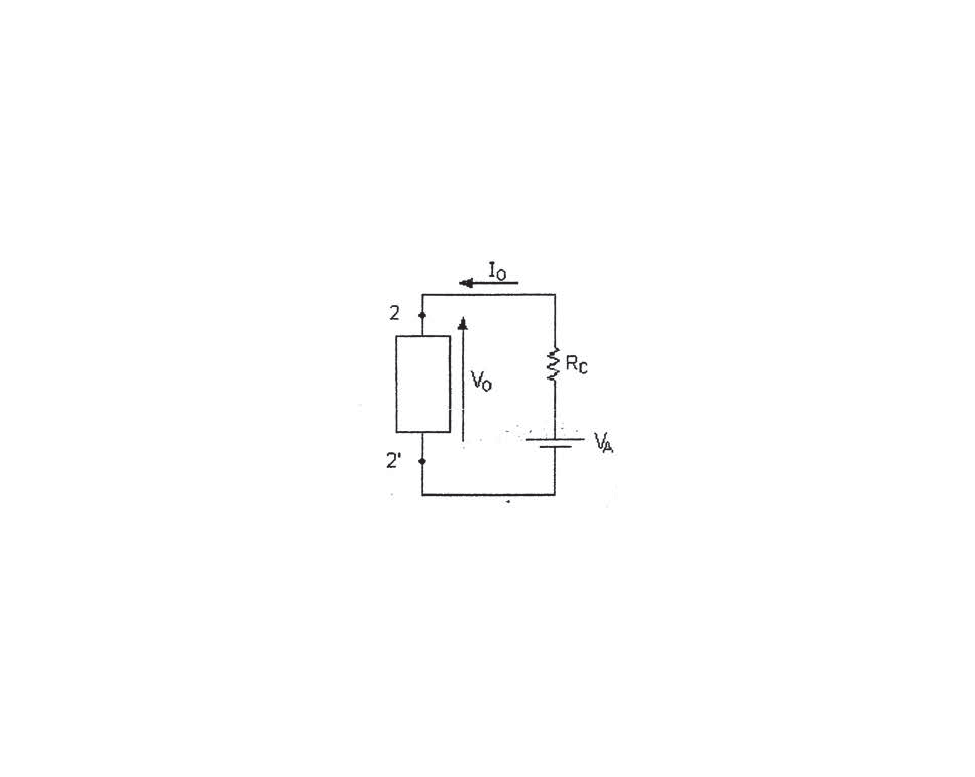
\includegraphics[scale=1]{figura0101.pdf}
    \caption{}
    \label{fig:1.1}
\end{figure}

La fuente de alimentación de tensión continua $V_A$, hará circular por la resistencia $R_C$ y el dispositivo una corriente continua $I_O$ que saldrá por el borne positivo de la fuente entrando al dispositivo por su terminal marcado como ``2''. Entre los terminales 2 y 2' existirá una diferencia de potencial de continua $V_O$. De acuerdo al sentido que se ha establecido para $I_O$, a los efectos de la fuente $V_A$ el dispositivo se comportará como un elemento pasivo de manera que la potencia entregada por $V_A$ se consumirá, parte en $R_C$ y parte en el dispositivo.

Este dispositivo posee además otro par de terminales 1-1' desde los cuales puede controlarse, \textbf{por medio de una tensión continua $V_I$ aplicada} entre ellos, \textbf{el valor de la corriente} $I_O$ que circula por los terminales 2-2' - Figura \ref{fig:1.2} -\footnote{Cabe acotar que según sea el principio físico de funcionamiento del dispositivo que se utilice, al aplicar una tensión $V_I$ entre el par de terminales de entrada o control, la corriente de entrada $I_I$ podrá ser nula o poseer un valor finito.}. 

De acuerdo con las condiciones de funcionamiento enunciadas para el dispositivo, diremos que el par de terminales 1-1' cumple la función de \textbf{par de terminales de entrada} al dispositivo, en tanto que 2-2' representa al \textbf{par de terminales de salida}, que entregan a la carga la corriente y tensión elaboradas por el dispositivo a partir de la tensión aplicada a los terminales de entrada.

\begin{figure}[!htbp]
    \centering
    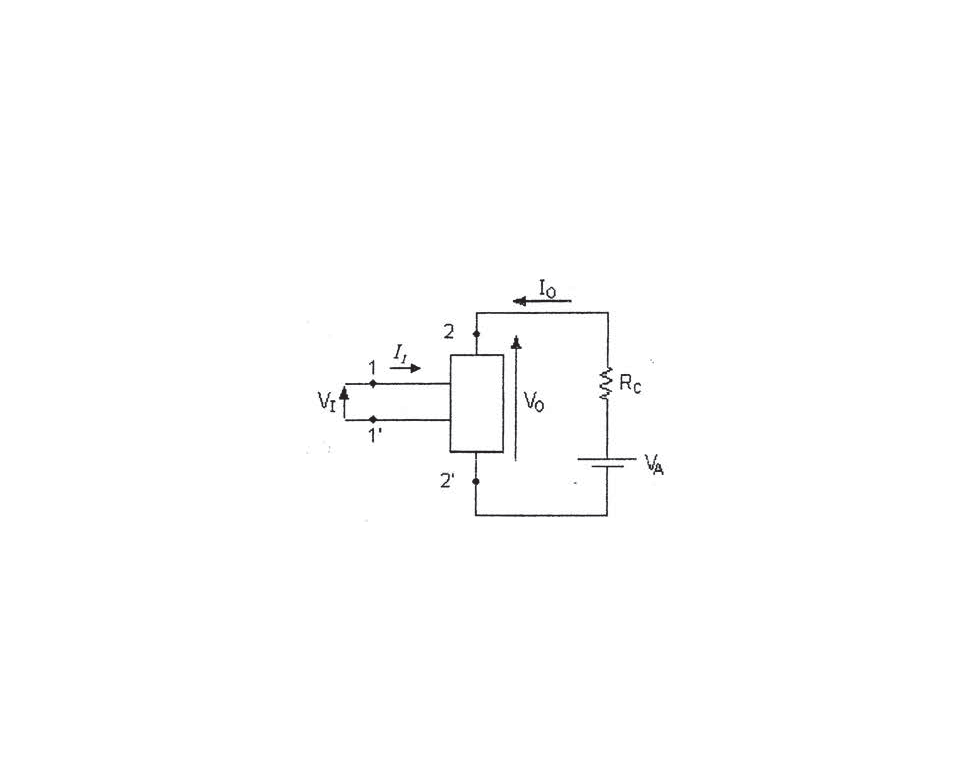
\includegraphics[scale=1]{figura0102.pdf}
    \caption{}
    \label{fig:1.2}
\end{figure}

Se admitirá considerando inicialmente un modelo básico de este dispositivo, que la corriente de salida $I_O$ \textbf{resulta proporcional a la tensión de entrada} $V_I$, y denominaremos $G_,$ a la \textbf{constante de proporcionalidad}, por lo que se podrá escribir:
\begin{equation}
    \label{eq:1.1}
    I_O=G_mV_I
\end{equation}
en donde $G_m=I_O/V_I$, posee dimensiones de conductancia y vincula una variable de salida ($I_O$) con una de entrada ($V_I$) por lo que se la denominará conductancia mutua o transconductancia. De este modo $G_m$ constituye la \textbf{transconductancia para corrientes y tensiones continuas} del dispositivos y será un valor constante (por haberse supuesto que es una constante de proporcionalidad), y por ende independiente de los valores de $I_O$ y $V_I$. Como $I_O$ depende sólo de $V_I$, de acuerdo a la definición dada del dispositivo, resultará independiente de $V_O$. Se considerará, para simplificar la explicación, que $G_m$ es positivo para los sentidos de referencia definidos para $I_O$ y $V_I$. El valor de $I_O$ queda determinado por lo tanto, \textbf{exclusivamente} por la tensión $V_I$. Se aceptará además que la ecuación (\ref{eq:1.1}) es válida sólo para valores positivo de $V_I$ (y por ende de $I_O$).

La tensión $V_O$ entre los terminales 2-2', resulta de la aplicación de la ley de Kirchoff de tensiones en la malla de salida del circuito:
\begin{equation}
    \label{eq:1.2}
    V_O=V_A-I_OR_C
\end{equation}

Formalmente, \textbf{la relación} $V_O/I_O$ representa el valor de una \textbf{resistencia equivalente para la continua, que presenta el dispositivo a la fuente $V_A$, para un valor} dado de la tensión de control $V_I$, dependiendo de ésta. Al aumentar la tensión $V_I$, se incrementará $I_O$, aumentando la caída de tensión en $R_C$ y disminuyendo en consecuencia $V_O$, con lo que disminuirá la resistencia equivalente que presenta el dispositivo a la fuente $V_A$.

Se mantendrá también la condición que el dispositivo definido siempre actuará como pasivo a los efectos de la tensión aplicada al circuito de salida, $V_A$, por lo que al variar el valor $V_I$, la corriente de salida $I_O$ y la tensión de salida $V_O$ se mantendrán siempre positivas de acuerdo a los sentidos de referencia adoptados en la figura \ref{fig:1.2}.

Si se representa la corriente de salida $I_O$ en función de la tensión de salida $V_O$, se obtendrá una \textbf{familia de rectas horizontales con $V_I$ como parámetro}, dado que $I_O$ no depende de $V_O$ de acuerdo a las particularidades con que se ha definido a este dispositivo. Estas curvas características de salida del dispositivo serán funciones de la forma:
\begin{equation}
    \label{eq:1.3}
    I_O=\left. f(V_O)\right|_{V_I=cte}
\end{equation}

El número de curvas $I_O=f(V_O)|_{V_I=cte}$, es decir con $V_I$ como parámetro, será infinito, una para cada uno de los valores que puede tomar $V_I$.

Tal como indica la expresión  (\ref{eq:1.1}), a iguales incrementos de $V_I$ corresponden iguales incrementos de $I_O$, por lo que al tomar incrementos iguales de $V_I$, las rectas horizontales $I_O=f(V_O)|_{V_I=cte}$ tendrán la misma separación en el eje $I_O$.

\begin{figure}[!htbp]
    \centering
    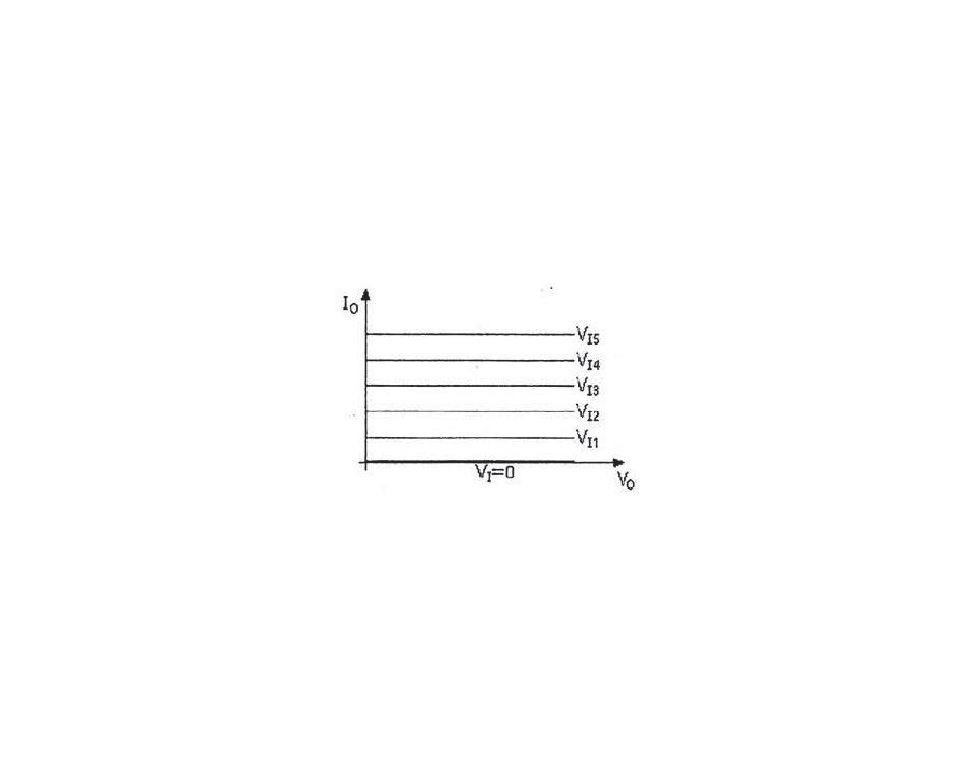
\includegraphics[scale=1]{figura0103.pdf}
    \caption{}
    \label{fig:1.3}
\end{figure}

La familia de rectas indicada en la figura \ref{fig:1.3} se denomina \textbf{características estáticas de salida del dispositivo} para valores de $V_I$ constantes, identificándose a la \textbf{tensión de control} $V_I$ como parámetro de entrada. Las características estáticas de salida con $V_I$ \textbf{como parámetro} representan el \textbf{lugar geométrico de los posibles pares de valores} ($I_O$, $V_O$) impuestos \textbf{por el dispositivo} al circuito exterior de la malla de salida.

De acuerdo a las consideraciones tenidas en cuenta al definir a este dispositivo, las características de salida deberán restringirse al primer cuadrante, ya que la potencia de continua entregada al dispositivo $V_A$, -$V_OI_O$- debe ser positiva (\textbf{potencia consumida} por el dispositivo entre sus terminales de salida, entregada por la fuente $V_A$).

Como la constante de proporcionalidad entre $I_O$ y $V_I$ se definió positiva para los sentidos de referencia indicados en la figura \ref{fig:1.2}, si se admite validez de la ecuación (\ref{eq:1.1}) para valores negativos de $V_I$, se tendrán valores negativos de $I_O$, por lo que será necesario que $V_O$ sea también negativa para que el dispositivo resulte pasivo a los efectos de $V_A$. En este caso, conservando todos los sentidos de la figura \ref{fig:1.2}, las curvas $I_O=f(V_O)|_{V_I=cte}$ estarán en el tercer cuadrante y serán válidas para valores negativos de $V_I$. En este caso, para que el conjunto del dispositivo que se ha definido y su circuito asociado pueden funcionar, deberá invertirse la fuente de alimentación $V_A$. 

\begin{figure}[!htbp]
    \centering
    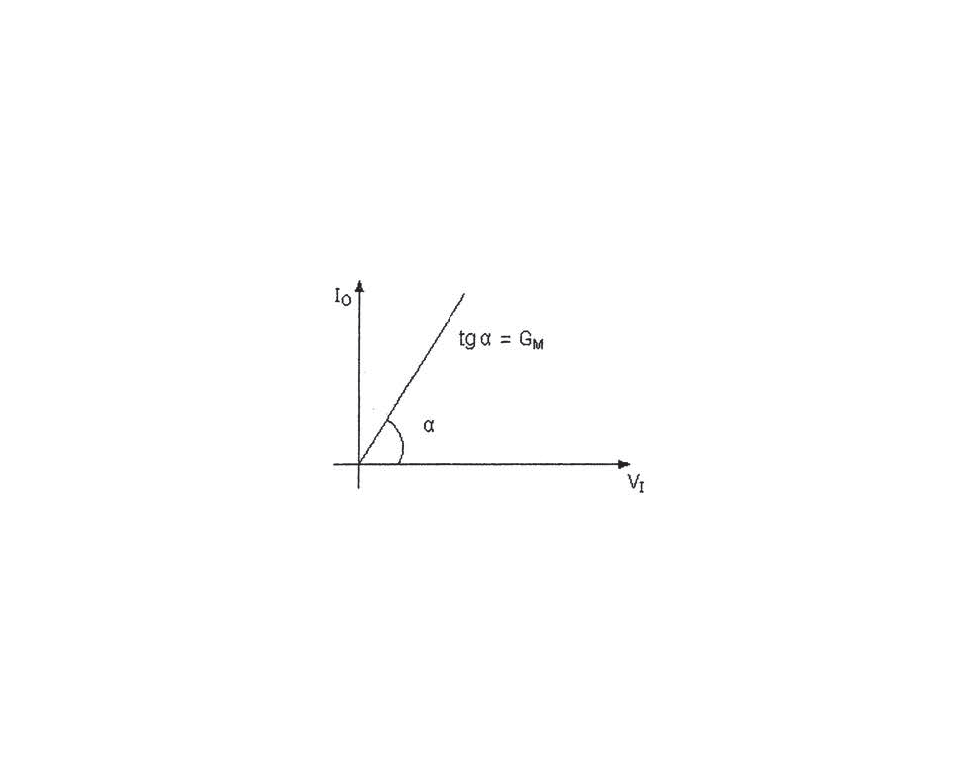
\includegraphics[scale=1]{figura0104.pdf}
    \caption{}
    \label{fig:1.4}
\end{figure}

La representación gráfica de la función $I_O=f(V_I)$, dada por la expresión (\ref{eq:1.1}), conduce a la característica más importante del tipo de dispositivo que se quiere introducir a partir de la definición dada. Esta es la \textbf{característica estática de transferencia directa}. Esta característica muestra la \textbf{acción de control}, que es el \textbf{principio} básico de acción del dispositivo definido. La figura \ref{fig:1.4} muestra esta característica que en este caso será una recta que pasa por el origen con pendiente $G_m$.

Si se conocen $V_A$, $R_C$ y $G_m$, puede determinarse el \textbf{punto de trabajo en continua} ``Q'' del dispositivo, definido por el \textbf{par de valores} ($I_{OQ}$, $V_{OQ}$), par un \textbf{dado valor de} $V_I(V_{IQ})$. Para encontrarlo, \textbf{analíticamente}, la solución se obtiene de la intersección de la característica de salida correspondiente al valor del parámetro $V_I=V_{IQ}$ y la recta que resulta de representar la ecuación (\ref{eq:1.2}) en el plano $I_O-V_O$ - figura \ref{fig:1.5}.

\begin{figure}[!htbp]
    \centering
    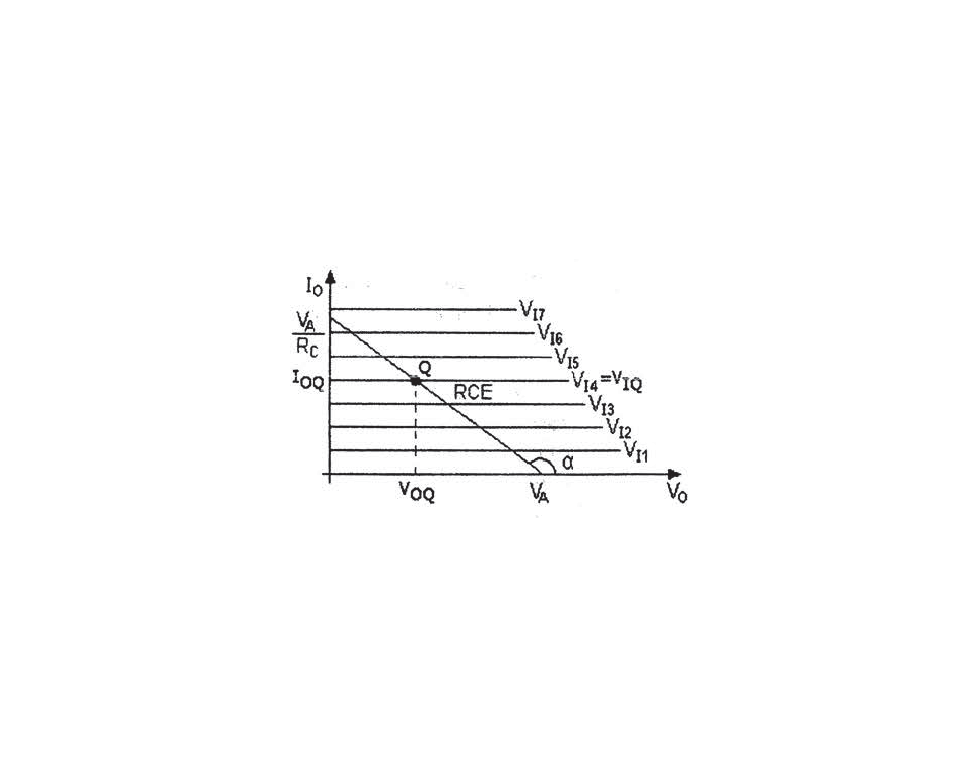
\includegraphics[scale=1]{figura0105.pdf}
    \caption{}
    \label{fig:1.5}
\end{figure}

Esta recta se denomina \textbf{recta de carga estática (RCE)} y representa el \textbf{lugar geométrico de los posibles pares de valores} ($I_O$,$V_O$) impuestos al dispositivo por el \textbf{circuito exterior de continua de la malla de salida}. La ecuación de la recta de carga estática se obtiene despejando $I_O$ en función de $V_O$ a partir de la ecuación (\ref{eq:1.2}) y tiene por \textbf{pendiente} a $\tan (\alpha) = -1/R_C$, \textbf{abscisa al origen} $V_A$ y \textbf{ordenada al origen} $V_A/R_C$:
\begin{equation}
    \label{eq:1.4}
    I_O=-V_O/R_C+V_A/R_C
\end{equation}

Si se modifica la tensión continua de control $V_I$, el punto de trabajo cambiará de ubicación, \textbf{manteniéndose siempre sobre la recta de carga}.

\begin{figure}[!htbp]
    \centering
    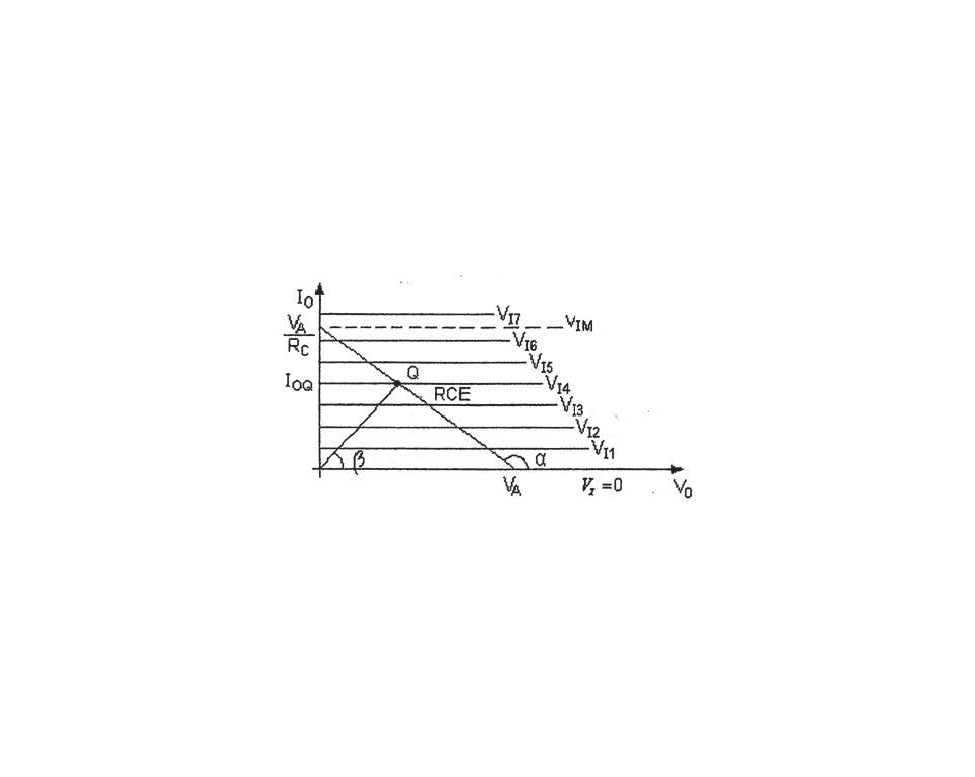
\includegraphics[scale=1]{figura0106.pdf}
    \caption{}
    \label{fig:1.6}
\end{figure}

\textbf{El punto de trabajo en continua (o estático) ``Q''} podrá tener cualquier ubicación sobre la recta de carga entre los límites dados por las intersecciones de esta con los ejes de coordenadas. Esto está de acuerdo con el hecho de que la ecuación (\ref{eq:1.1}) es válida en el primer cuadrante. De este modo la corriente $I_O$ podrá tomar como valor mínimo $I_{Om}=0$ y el valor máximo $I_{OM}=V_A/R_C$, como se ve en la figura \ref{fig:1.7}

Para valores de $V_I$ menores que cero o mayores que $I_{OM}/G_m$ se admitirá que el punto de trabajo permanecerá en uno de los puntos extremos definidos. En resumen, $V_I$ \textbf{tendrá posibilidades de controlar la corriente de salida} $I_O$, solo mientras se cumpla $0\leq V_I \leq V_{IM}$ que se denomina \textbf{rango de control de la variable de entrada}. Fuera de este rango, $V_I$ pierde la propiedad de controlar a $I_O$ y el punto Q se ubicará con corriente de salida nula y tensión $V_A$ para todo $V_I\leq 0$ y en la posición de tensión de salida nula y corriente $V_A/R_C$ para todo $V_I\geq I_{OM}/G_m$.

\begin{figure}[!htbp]
    \centering
    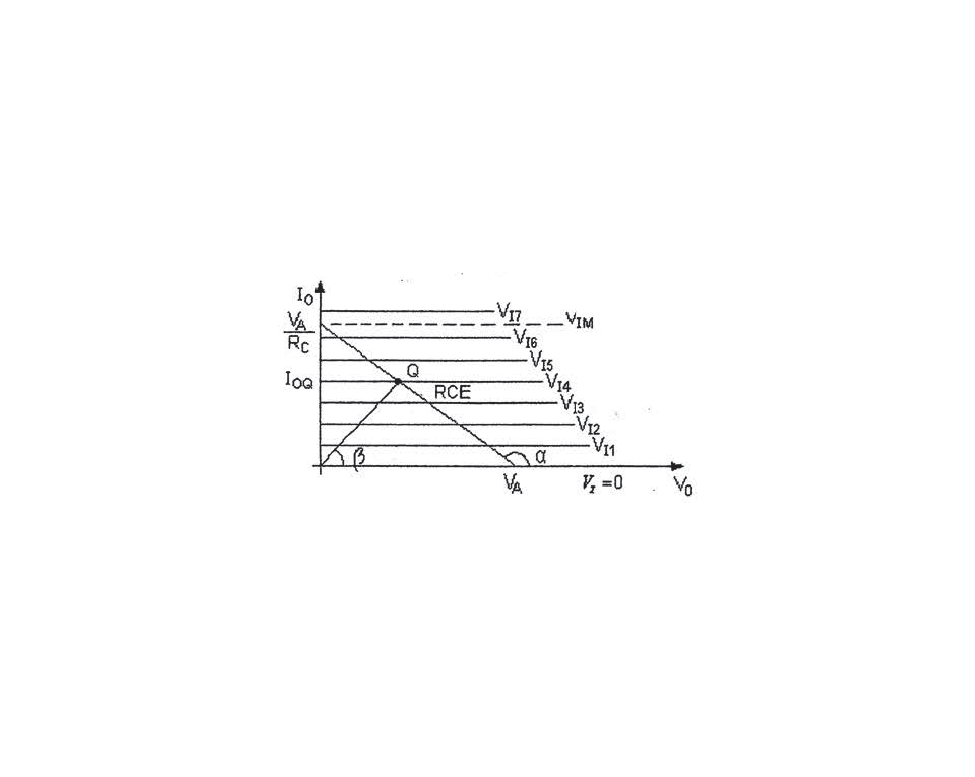
\includegraphics[scale=1]{figura0107.pdf}
    \caption{}
    \label{fig:1.7}
\end{figure}

\textbf{Gráficamente}, se ve que \textbf{al variar $V_I$ varía} el valor del ángulo $\beta$ de acuerdo a la relación de $I_O$ von $V_O$, es decir, se modifica \textbf{el valor de la resistencia estática de salida $R_{EO}$} dada por la \textbf{la relación $V_O/I_O$}, como se desprende de la figura \ref{fig:1.7} donde se cumple que $\tan (\beta) = 1/R_{EO}$\footnote{La resistencia estática de salida, para un valor determinado de $V_I$, se define colocando un generador de tensión continua ideal entre los terminales de salida del dispositivo \textbf{como tensión de prueba} $V_{Op}$ y hallando la relación entre la tensión de prueba y la corriente que esta produce $R_{EO}=\left. V_{Op}/I_{Op}\right|_{V_I=cte}$ (equivalente a conectar un óhmetro entre los terminales 2-2').}, para el punto de trabajo correspondiente a cada valor de la tensión de entrada $V_I$. Es decir, variando la tensión de control $V_I$ se esta variando la resistencia estática de salida $R_{EO}$ del circuito. Esto equivale a que, desde el circuito de entrada, se transfiere a la malla de salida, una resistencia variable, cuyo valor se controla mediante la tensión de entrada $V_I$. De este modo, surge que el funcionamiento del dispositivo definido, se basa en obtener una \textbf{resistencia estática variable a la salida, cuyo valor se transfiere} desde la entrada partir de las variaciones del parámetro de control. A este resultado se lo denomina \textbf{efecto transistor}.

\begin{figure}[!htbp]
    \centering
    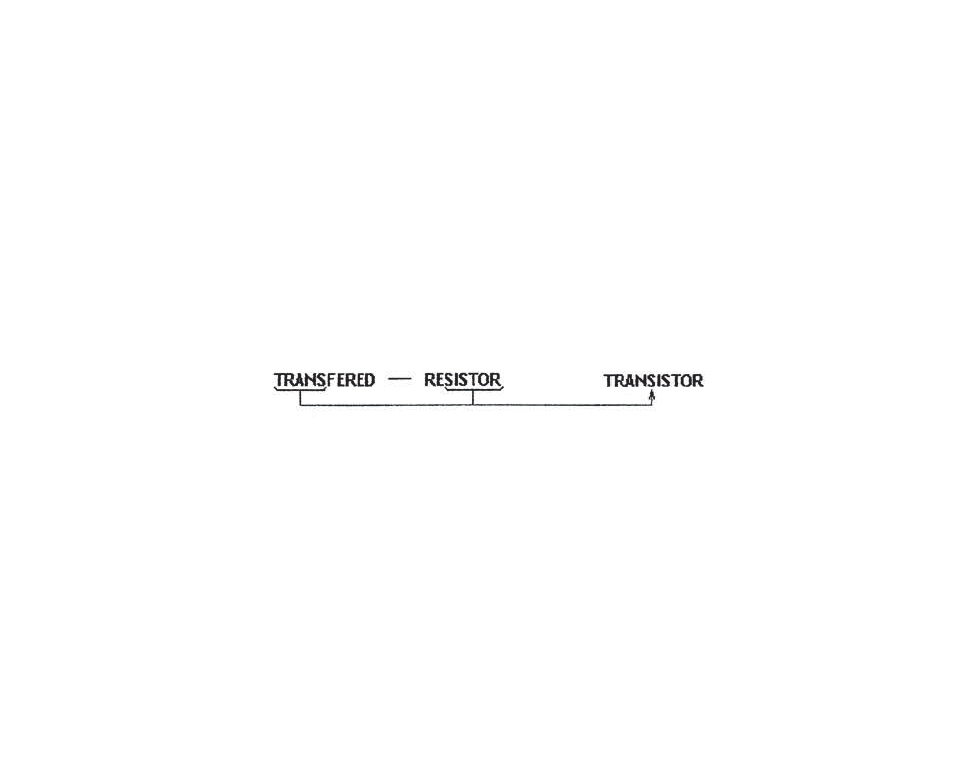
\includegraphics[scale=1]{figura0108.pdf}
\end{figure}

\chapter{Base de funcionamiento de los dispositivos amplificadores}

\section{Modos de funcionamiento}
El dispositivo de control de señal bajo estudio, que ya llamaremos \textbf{transistor}, puede trabajo en \textbf{dos modos de funcionamiento} claramente diferenciados: modo \textbf{digital} y modo \textbf{analógico}.

\subsection{Funcionamiento del dispositivo en modo digital}
En el modo digital, $V_I$ podrá tomar valores tales que el punto de trabajo se encuentre sólo en dos puntos determinados de la recta de carga estática, generalmente en uno u otro extremo de ella, pues allí teóricamente no existe disipación de potencia.

Para $V_I$ nulo o negativo (de acuerdo con los sentidos adoptados), el punto de trabajo estará en el extremo inferior de la RCE donde $I_O=0$ y $V_O=V_{A}$, resultando infinita la resistencia que presenta el dispositivo a la carga (equivalente a una llave abierta). En este caso se dirá que el dispositivo está \textbf{al corte}. Si $V_I$ es tal que la corriente $I_O$ sea igual a $V_A/R_C$, el punto de trabajo se ubica en el extremo superior de la RCE con $I_O=V_A/R_C$ y $V_O=0$, de donde la resistencia que presenta el dispositivo a la carga resulta nula (equivalente a una llave cerrada). En este caso se dirá que el dispositivo está \textbf{saturado}, ya que la corriente $I_O$ no puede seguir aumentando aunque lo haga $V_I$.

Para este modo de operación el dispositivo puede representarse como se indica en la figura \ref{fig:2.1}, donde \textbf{la condición de llave abierta o cerrada se comanda por medio de la tensión de control $V_I$.}

\begin{figure}[!htbp]
    \centering
    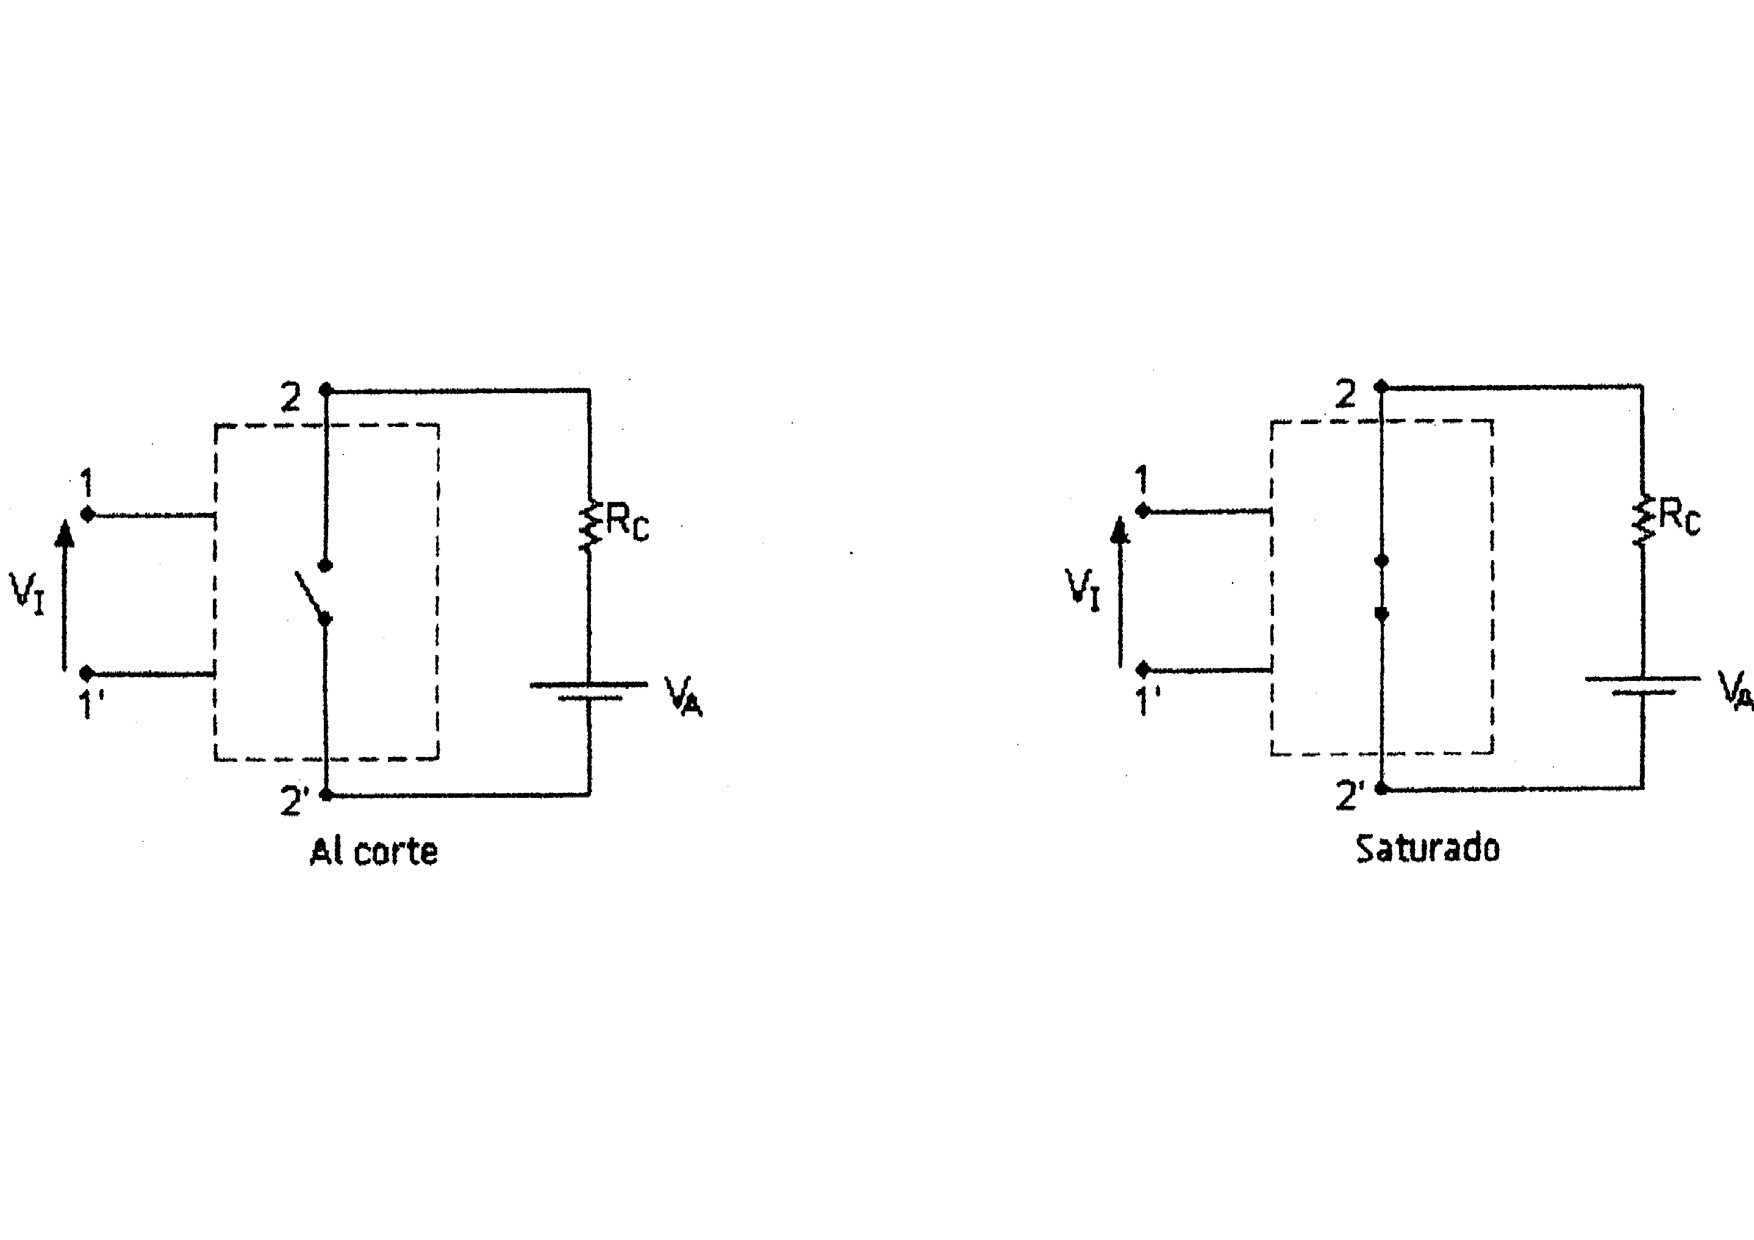
\includegraphics[width=\textwidth]{figura0201.pdf}
    \caption{}
    \label{fig:2.1}
\end{figure}

Entonces, en el modo de operación digital, el dispositivo trabajará al corte o saturado. Es de hacer notar que \textbf{en ninguno de los casos el dispositivo disipa potencia}.

\subsection{Funcionamiento del dispositivo en modo analógico}

En \textbf{modo analógico} la señal de control $V_I$ toma \textbf{cualquiera de los infinitos valores comprendidos entre 0 e $I_{OM}/G_m$}. En este caso la tensión aplicada entre los terminales de entrada del dispositivo \textbf{podrá ser una tensión continua o variable en el tiempo}. Tomaremos para nuestro estudio un caso particular en que la tensión de entrada esta compuesta por una continua a la que se superpone una señal que varía en el tiempo. De aquí en adelante denominaremos $V_I$ para la componente continua e indicando con $v_i$ a la señal que varía en el tiempo a su alrededor:
\begin{equation}
    \label{eq:2.1}
    v_I=V_I+v_i
\end{equation}

Entenderemos por \textbf{señal aplicada}, a una tensión (o corriente) que varía en el tiempo resultando un incremento (positivo, negativo o periódico con semiciclos de ambos signos) de la tensión total $v_I$. Este incremento podrá ser un escalón de tensión del tipo:
\begin{equation}
    \label{eq:2.2}
    v_i=V_i\cdot u(t)
\end{equation}
o una tensión que varía en el tiempo en forma periódica o no.

Con \textbf{base conceptual en el desarrolla de Fourier}, resulta de suma facilidad para comprender la propiedad fundamental del funcionamiento de los dispositivo de control de señal en un circuito, considerar que $v_i$ varía senoidalmente en el tiempo:

\chapter{Análisis de pequeña señal de circuitos amplificadores}

\chapter{Estudio de los Parámetros Característicos de Circuitos Amplificadores. Análisis por inspección.}

\chapter{Otros parámetros característicos de circuitos amplificadores}

\chapter{Estabilidad del punto de reposo}

\chapter{Nociones de realimentación para señal. Análisis para el rango de frecuencias medias.}

\chapter{Introducción al análisis de respuesta en frecuencia}

\part{Complementos sobre temas circuitales}

\chapter{Polarización y funcionamiento con señal en circuitos de un transistor}

\chapter{Análisis en pequeña señal de circuitos con un solo transistor y sus distintas configuraciones}

\chapter{Etapa con un transistor bipolar en emisor común con acople directo de la resistencia de carga}

\chapter{Etapa con dos generadores de excitación}

\chapter{Limitaciones en el uso de transistores bipolares}

\chapter{Principios básicos de amplificadores con varios transistores}

\chapter{Estudio de circuitos R-C}

\chapter{Respuesta en frecuencia de circuitos amplificadores}

\chapter{Amplificadores diferenciales y fuentes de corriente}

\chapter{Amplificadores diferenciales con carga activa}

\chapter{Amplificadores operacionales: Conceptos básicos}

\part{Problemas}

\chapter{Conceptos generales de circuitos analógicos y de conmutación}

\chapter{Estudio de polarización y estabilidad de amplificadores con un solo transistor}

\chapter{Estudio de la respuesta en frecuencia de amplificadores con un transistor}

\chapter{Estudio del comportamiento de amplificadores con más de un transistor a frecuencias medias}

\chapter{Estudio de la respuesta en frecuencia de amplificadores con varios transistores}

\chapter{Amplificadores diferenciales, fuentes de corriente y cargas activas}

\part{Apéndices}
\begin{appendices}
\chapter{Semiconductores, junturas y dispositivos sólidos activos}

\section{Semiconductores}

\subsection{Introducción}
Para poder explicar la física de los semiconductores (germanio, silicio o materiales compuestos, como arseniuro de galio, fosfuro de galio, carburo de silicio, etc.) podemos utilizar dos modelos diferentes:

El primer modelo es de análisis cualitativo y se lo conoce como \emph{modelo de enlaces}. En la estructura diamante del germanio y del silicio cada átomo forma cuatro enlaces covalentes con los cuatro átomos que lo rodean. Para romper una unión y que surja un electrón libre, debemos comunicar energía al sólido, lo que implica subir la temperatura. A $T>0^\circ K$, al romperse una unión, surge un electrón libre animado de energía de agitación térmica que lo hace moverse al azar. El lugar que deja el electrón se lo denomina laguna o hueco. Este hecho provoca una no neutralidad eléctrica, por lo que un electrón ligado de un enlace cercano puede introducirse en el lugar vacante, dejando a su vez un nuevo hueco. Es decir, todo sucede como si una partícula de carga positiva se hubiese desplazado en sentido contrario al movimiento del electrón. Podemos decir entonces que la conducción en un semiconductor se debe tanto a una corriente de electrones libres como de lagunas.

El segundo modelo, es de análisis cuantitativo y se lo conoce como \emph{modelo de bandas}. Si tengo dos átomos separados con un mismo nivel de energía permitido, puedo tener dos electrones en cada átomo, debido al spin. Cuando se van acercando, por el principio de exclusión de Pauli, dicho nivel deberá desdoblarse en dos subniveles. En el caso de tener N átomos con un mismo nivel de energía permitido, dicho nivel se desdoblará en N niveles, formando una banda de energía cuasi continua (dada la gran cantidad de átomos que interactúan), donde se ubicarán los 2N electrones \footnote{Dado un sólido de distancia interatómica ``a'', su diagrama de bandas es equivalente a hacer un corte en el diagrama de distribución de niveles de energía a una distancia ``a''.}. 

La densidad de corriente $J$, será $J=q\sum v_i$, donde se sumarán todos los electrones de la banda por unidad de volumen. Tanto en una banda vacía, como en una llena, $J=0$. En una banda casi vacía, la corriente estará dada por los electrones que pasaron a los niveles permitidos superiores por ser más energéticos. Mientras que una banda casi llena, la corriente puede ser expresada por la producida por los estados vacantes, tratados como  partículas de carga positiva (huecos).

En los semiconductores, entre la última banda llena (cuyo nivel superior se denomina energía de valencia, $E_v$) y la primera vacía (cuyo nivel inferior se lo denomina energía de conducción, $E_c$), habrá una zona de energía prohibida o ``gap'', $E_g=E_c-E_v$. Los semiconductores poseen valores de $E_g$ entre $0.5 eV$ y $5 eV$. Valores superiores de $E_g$ corresponden a materiales aisladores.

\subsection{Semiconductores en equilibrio}

Un semiconductor se encuentra en \emph{equilibrio térmico}, cuando se encuentra a temperatura constante en el tiempo y uniforme en el espacio y ningún agente físico o químico externo actúa sobre él, salvo el intercambio térmico con el medio ambiente. En este caso, si cada proceso que ocurre en el material se encuentra contrarrestado por otro proceso opuesto, se dice que se encuentra en \emph{equilibrio termodinámico}.

En este caso, la generación térmica de pares electrón-hueco por unidad de tiempo y de volumen (excitación de un electrón desde la banda de valencia a la de conducción) resulta igual a la recombinación térmica de pares por unidad de tiempo y de volumen (desexcitación de un electrón desde la banda de conducción a la de valencia).

La generación dependerá de la temperatura, mientras que la recombinación dependerá también de la concentración de electrones ``n'' en la banda de conducción y de la concentración ``p'' de huecos en la banda de valencia, dado que ambos deben interactuar para que la recombinación ocurra: 
\[g=f_1(T)=r=n\cdot p\cdot  f_2(T)\Rightarrow n\cdot p =f_3(T)\]

Es decir, el productor de las concentraciones de electrones y huecos en un dado semiconductor en equilibrio térmico es sólo función de la temperatura.

Si aplicamos esta afirmación para un semiconductor puro o intrínseco\footnote{Se considera intrínseco cuando tiene hasta 1 átomo de impureza por cada $10^{10}$ átomos de semiconductor. Cada electrón excitado a la banda de conducción deja un hueco en la banda de valencia. Es decir, los electrones y huecos se crean de a pares.}, donde $n=p=n_i$, entonces $n_i^2=f_3(T)$, y como la concentración intrínseca es constante para un semiconductor a una dada temperatura, es posible reemplazar $n_i$ para obtener $n\cdot p =n_i^2$ (ecuación válida para semiconductores intrínsecos o extrínsecos en equilibrio termodinámico).

\subsection{Semiconductores extrínsecos}

La forma más usada de controlar el numero de portadores en un semiconductor, es incorporando impurezas que ocupan en la red cristalina el mismo lugar del átomo substituido.

Supongamos que agregamos impurezas correspondientes al grupo V de la tabla periódica (5 electrones de valencia). El quinto electrón estará unido por unión covalente como los oros cuatro con átomos vecinos del semiconductor. Sólo se encuentra unido al átomo de impurezas por un excesos de carga positiva del núcleo. Con una pequeña cantidad de energía ($T>0^\circ K$) este quinto electrón puede romper su enlace electrostático y convertirse en electrón libre, dejando un ión positivo. Este tipo de impurezas se denominan donoras.

Si agregamos impurezas correspondientes al grupo III (3 electrones de valencia), los tres electrones de valencia se unirán por enlaces covalentes con tres átomos vecinos de semiconductor, dejando un enlace vacante. Con una pequeña cantidad de energía ($T>0^\circ K$), un electrón de un enlace covalente vecino puede ocupar dicho enlace vacante y crear laguna, dejando negativo al ión de impureza. Este tipo de impurezas se denominan \emph{aceptoras}.

Un semiconductor con impurezas donoras o aceptoras, se lo denomina extrínseco. 

Cuando el número de átomos donores por unidad de volumen, $N_D$, es mayor que el de aceptores, $N_A$, se dice que el semiconductor es de tipo N. en el caso opuesto, se dice que es de tipo P. Ambas cantidades deberán ser mucho menores que el número total de átomos del  semiconductor ($10^{22}$ átomos$/cm^3$), en caso contrario se dice que el material se encuentra degenerado y pierde sus propiedades de monocristal para transformarse en cristal amorfo.

Entonces, existen dos formas para obtener portadores libres en un semiconductor: por generación térmica en átomos propios o por ionización de átomos de impurezas.

Supongamos un semiconductor tipo N, fuertemente contaminado o \emph{dopado mayoritariamente} con $N_D\gg n_{\textrm{generación intrínseca}}$ y $N_A=0$. Podemos decir que por encima de los $200^\circ K$, ya todos los átomos de impureza están ionizados (los componentes semiconductores trabajarán normalmente entre $200$ y $450^\circ K$). Entonces, la cantidad de electrones libres estará dada por:
\[n=n_{\textrm{átomos de impurezas}}+n_{\textrm{generación intrínseca}}\simeq N_D\]

Mientras que la cantidad de huecos corresponderá sólo a la generada térmicamente (pues la generación intrínseca produce de a pares electrón-hueco):
\[p=p_{\textrm{generación intrínseca}}=n_{\textrm{generación intrínseca}}\leq n_i\]

Podemos concluir que, bajo estas condiciones típicas, la concentración de portadores mayoritarios es prácticamente constante, mientras que la de minoritarios depende fuertemente de la temperatura.

\subsection{Conductividad}

En un cristal, a temperaturas mayores que $0^\circ K$, los electrones y los huecos son partículas casi libres en el sentido que no están asociados a ningún sitio en particular de la red y se mueven aleatoriamente colisionando con la red (con un tiempo libre medio entre colisiones) a la cual le entregan energía en casa proceso de choque.

Cuando aplicamos un campo eléctrico $E$ sobre el cristal, en promedio los electrones se deslizarán en sentido contrario al campo con una velocidad de corrimiento $v_c$.

La densidad de corriente que fluye en la dirección del campo será:
\[J_n=n\cdot q\cdot \mu_n\cdot E\]

La \emph{movilidad} $\mu_n$ describe la facilidad con la que un electrón se mueve bajo la acción de un campo aplicado.

Haciendo un análisis similar con los huecos, se obtiene que la densidad de corriente total será la suma de la de huecos y electrones:
\[J=q\cdot (n\cdot  \mu_n + p\cdot \mu_p)\cdot E=\rho \cdot E\]

La \emph{conductividad} $\rho$ representa la facilidad con que el campo genera una densidad de corriente en un material.

En un semiconductor la movilidad de los electrones es mayor que la de los huecos (3 veces más en Si), ya que resulta más fácil comunicarme movimiento a un electrón libre que a uno ligado, cuyo desplazamiento provocara el desplazamiento de la laguna. En Si, $\mu_n=1350 c^2/Vseg$ y en GaAs, $\mu_n=8500 cm^2/Vseg$.

La movilidad disminuye al aumentar la temperatura, ya que el aumento de la vibración de los átomos de la red cristalina, aumenta la superficie efectiva de choque, disminuyendo el tiempo entre colisiones. También disminuye al aumentar la concentración, ya que los átomos de impurezas agregadas al cristal producen distorsiones locales en la red, lo cual produce un aumento de la dispersión de los portadores libres.

Normalmente, la movilidad de electrones libres en un semiconductor es algo mayor que la existente en un metal (unas 10 veces), ya que las distancias interatómicas son menores que en el semiconductor, aumentando la probabilidad de choque (menor tiempo libre medio entre colisiones). Por otro lado, como el número de portadores libres en un metal es muy superior a los de un semiconductor (unas 1000 veces), la conductividad en un metal será siempre mucho mayor que en un semiconductor.

Para analizar la variación de la conductividad con la temperatura, podemos hacer una comparación entre el metal y el semiconductor. En el conductor, existen un solo tipo de portadores: electrones. Por lo tanto, $\rho_M=q\cdot \mu_n\cdot n$. La densidad de electrones libres permanecerá constante con la temperatura, por lo que la conductividad disminuirá como lo hace la movilidad.

Por otro lado, en un semiconductor extrínseco:
\[\rho_S=q\cdot(n\cdot \mu_n+p\cdot \mu_p)\]

Obteniéndose, para un Si tipo N, la siguiente gráfica de variación de la concentración con la temperatura:
\begin{figure}[!htbp]
    \centering
    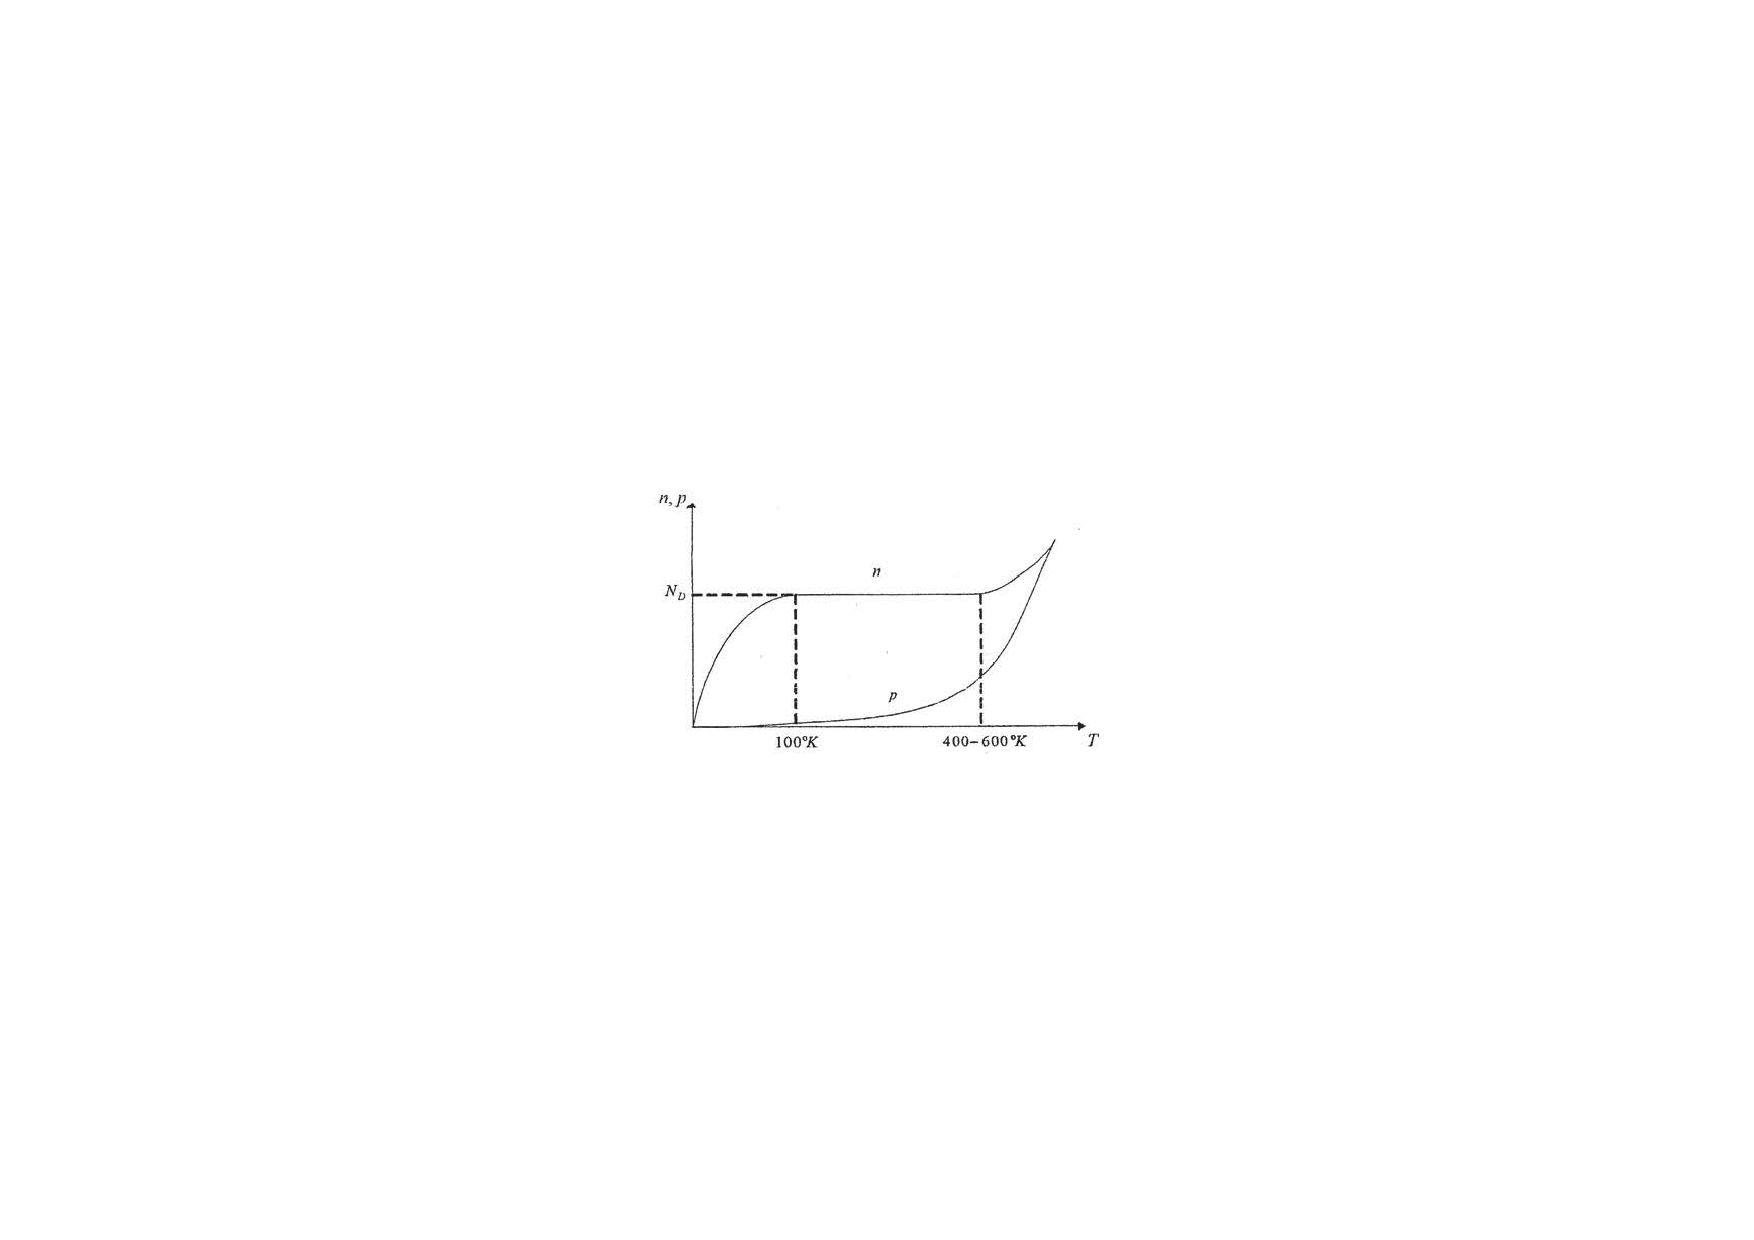
\includegraphics[width=\textwidth]{figuraa01.pdf}
    \caption{}
    \label{fig:a.1}
\end{figure}

Con lo que se puede inferir que la conductividad disminuirá con la temperatura igual que la movilidad mientras la concentración permanezca constante, aumentando luego a partir de $400^\circ K$ a $600^\circ K$, cuando la generación térmica deje de ser despreciable.

\subsection{Ecuación de continuidad}

Mediante el planteo de esta ecuación se obtendrán todas las expresiones relacionadas con la corriente en semiconductores. Es una ecuación general que plantea el principio de conservación de la carga eléctrica y se escribe en base a las siguientes consideraciones:
\begin{enumerate}
	\item En un semiconductor extrínseco siempre se planteará para los portadores minoritarios, pues éstos son los que ponen de manifiesto los fenómenos de generación y recombinación.

	\item Consideramos válida la hipótesis de cuasi neutralidad por la cual, si existe una densidad de carga neta en el material, es despreciable frente a la concentración de portadores mayoritarios y el material puede considerarse prácticamente neutro. Es decir que podemos admitir que los excesos de portadores mayoritarios y minoritarios son iguales. Sin embargo, el exceso de minoritarios en relación con la concentración de equilibrio es mucho mayor que el exceso de mayoritarios en relación con su concentración de equilibrio. Es decir, la concentración de mayoritarios no se ve afectada: \emph{condición de bajo nivel de inyección}.
\end{enumerate}

\section{Juntura P-N: Diodos}

\subsection{Juntura P-N en equilibrio termodinámico}

Existen dos técnicas principales para la construcción de junturas: P-N:
\begin{itemize}
	\item Epitaxial: se parte de un semiconductor base P o N y se construye el otro material del tipo opuesto por una deposición de átomos. De esta forma se logra que la concentración de ambos materiales sea uniforme y que la juntura obtenida sea abrupta (es decir, la contaminación sufre un salto de muy alta pendiente de la concentración donora a la aceptora).

	\item Compensación: consiste en difundir un tipo de impureza (donora o aceptora) sobre un material de tipo opuesto. En este caso no se obtiene una juntura abrupta, sino gradual.
\end{itemize}

Para simplificar el análisis, tomaremos el caso de la juntura abrupta. Supongamos que tenemos dos materiales de contaminación uniforme tipos N y P. Admitamos que el material P está más contaminado que el N, es decir $N_A>N_D$, (se suele escribir como materiales de tipo P\textsuperscript{+} y N).

Al unir estos dos materiales, por la diferencia de concentraciones existente en la zona de unión, los electrones del lado N se difundirán hacia el lado P\textsuperscript{+} y los huecos del lado  P\textsuperscript{+} se difundirán hacia el N, dejando en la zona cercana al plano de unión, iones positivos y negativos, respectivamente, sin neutralizar. Dichos portadores mayoritarios, al difundirse a través de la juntura, se convertirán en minoritarios en exceso del lado opuesto y por lo tanto ser recombinarán rápidamente con los mayoritarios, quienes al recombinarse dejan a su vez iones de átomos de impurezas sin neutralizar. Se forma entonces una \emph{zona desierta} de portadores libres en los alrededores del plano de unión. 

El proceso seguirá hasta que la carga de los iones fijos sin compensar a ambos lados de la unión (positiva del lado N y negativa del lado P) provoque un campo eléctrico tal que cause una tendencia al corrimiento igual y opuesta a la tendencia a la difusión.

\begin{figure}[!htbp]
    \centering
    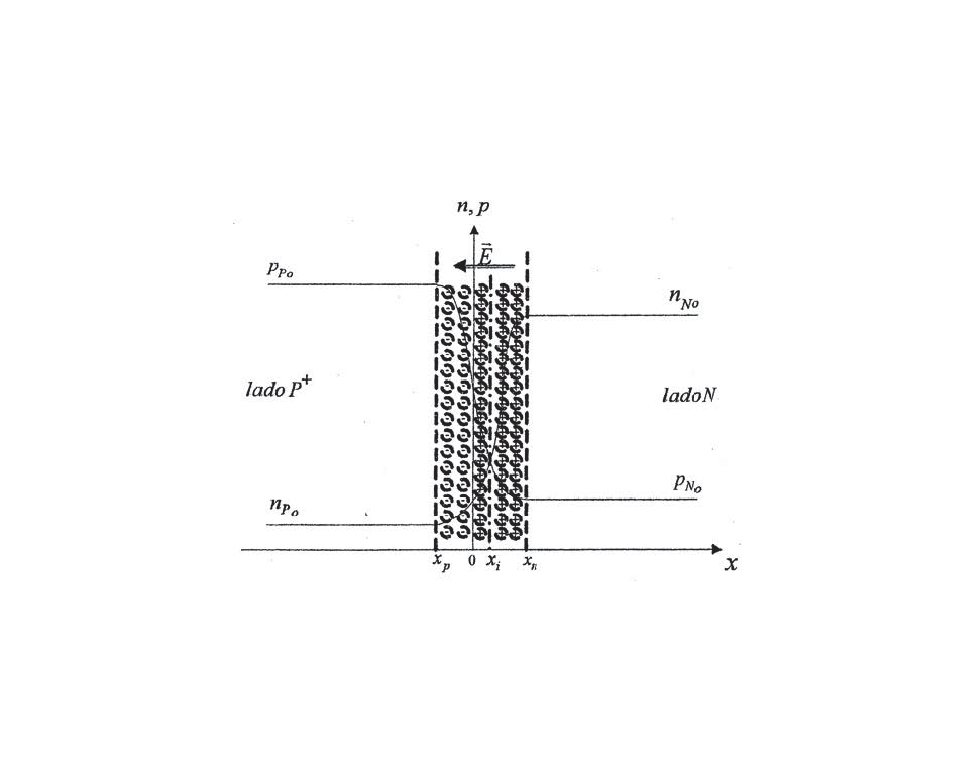
\includegraphics[scale=1]{figuraa02.pdf}
    \caption{}
    \label{fig:a.2}
\end{figure}

Obviamente, por el principio de conservación de la carga eléctrica, el nuevo material así unido sigue siendo eléctricamente neutro. Y como las cargas de los iones de ambos lados deben igualarse, la zona desierta será más extensa del lado del material menos dopado.

Como puede verse en la figura \ref{fig:a.2}, la hipótesis de la existencia de una zona de deserción total resulta válida, pues la concentración de mayoritarios en los alrededores de la unión desciende bruscamente. Fuera de esta zona desierta, los materiales se suponen perfectamente neutros.

\subsection{Juntura P-N con polarización}

Para polarizar una juntura, es decir, aplicarle una diferencia de potencial, es necesario construir contactos del tipo metal-semiconductor, tanto del lado P como del N. Dichos contactos se clasifican en dos tipos\footnote{Para una explicación más detallada sobre contactos M-S, referirse al apéndice B.}:
\begin{itemize}
	\item 
\end{itemize}






\chapter{Juntura Metal-Semiconductor}
\chapter{Introducción a circuitos con diodos}
\section{Características Estáticas de Dispositivos}
Consideremos un dispositivo de dos terminales que denominaremos ``X'', que puede presentar tanto efectos reactivos como disipativos. La característica estática del dispositivo será una curva donde se lleve la corriente que lo atraviesa $I_x$ en función de la tensión aplicada externamente entre los dos bornes del dispositivo $V_x$. Para obtenerla experimentalmente deberán medirse cierta cantidad de pares de valores ($I_x$, $V_x$), los cuales podràn o no estar relacionados por una expresión conocida.

La figura \ref{fig:c.1} muestra un posible circuito de medición, en el cual la resistencia $R$ se coloca a fin de limira la corriente máxima por el circuito -en particular cuando el dispositivo ``X'' presenta grandes aumentos de corrientes ante pequeños incrementos de tensión 

\begin{figure}[!htbp]
\centering
\begin{minipage}{.5\textwidth}
  \centering
  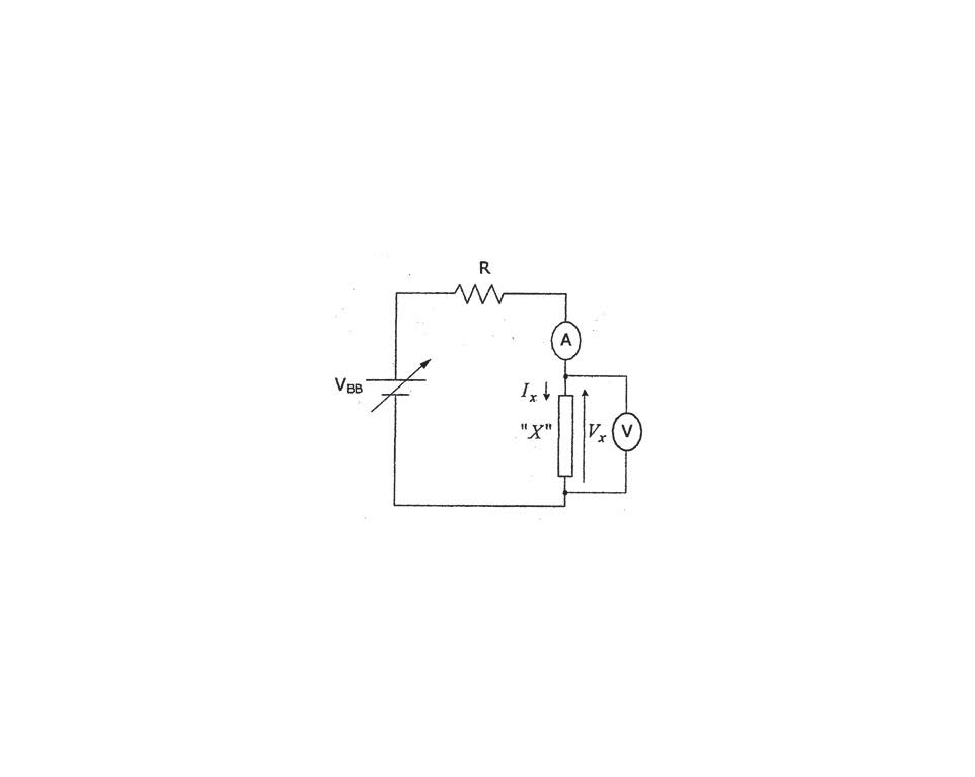
\includegraphics[scale=1]{figurac01.pdf}
  \captionof{figure}{}
  \label{fig:c.1}
\end{minipage}%
\begin{minipage}{.5\textwidth}
  \centering
  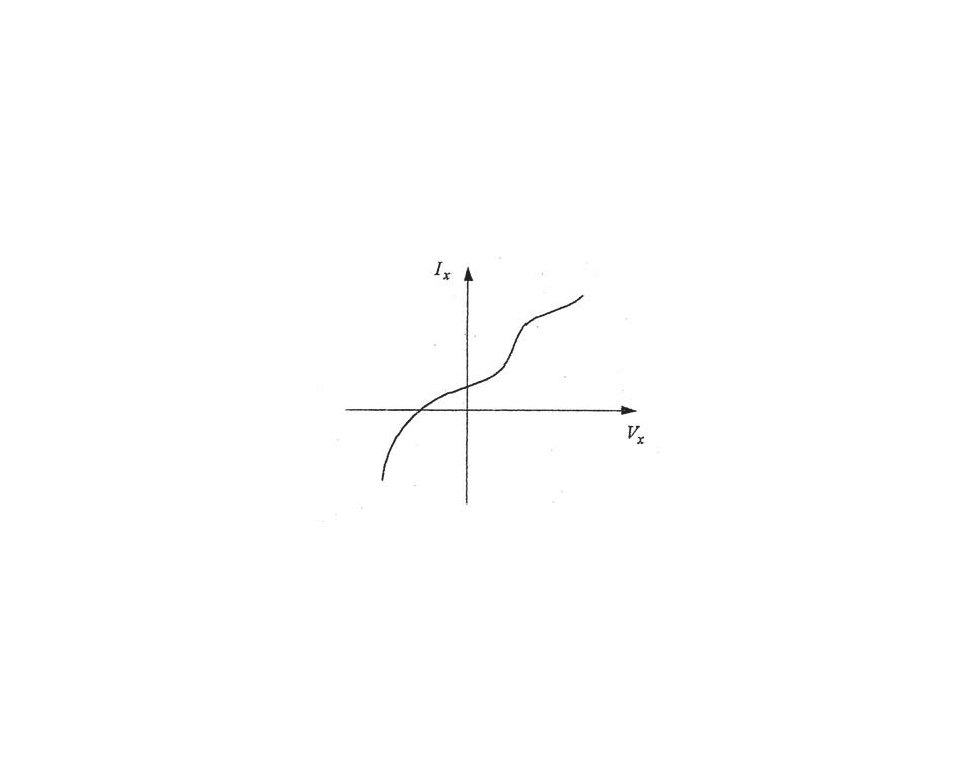
\includegraphics[scale=1]{figurac02.pdf}
  \captionof{figure}{}
  \label{fig:c.2}
\end{minipage}
\end{figure}

Cada par de valores deberá ser medido de una vez que se hayan extinguido todos los transitorios producidos luego de cada incremento de $V_{BB}$ entre dos mediciones sucesivas. De ahí la denominación de \emph{característica estática}, lo cual implica que los efectos reactivos no influyen en su trazado.

Definimos entonces como característica estática de un dispositivo de dos terminales al conjunto de valores estáticos ($I_x$, $V_x$), que son compatibles con el funcionamiento del dispositivo - figura \ref{fig:c.2}.

\begin{exmp}
Si el dispositivo es un resistor lineal e invariante en el tiempo, su característica estática será una recta determinada por la ley de Ohm $I_x=I_R=V_R/R=V_x/R$ - figura \ref{fig:c.3} -. Esta característica resulta válida dentro de límites prefijados de tensión y corriente dados por el fabricante.

\begin{figure}[!htbp]
    \centering
    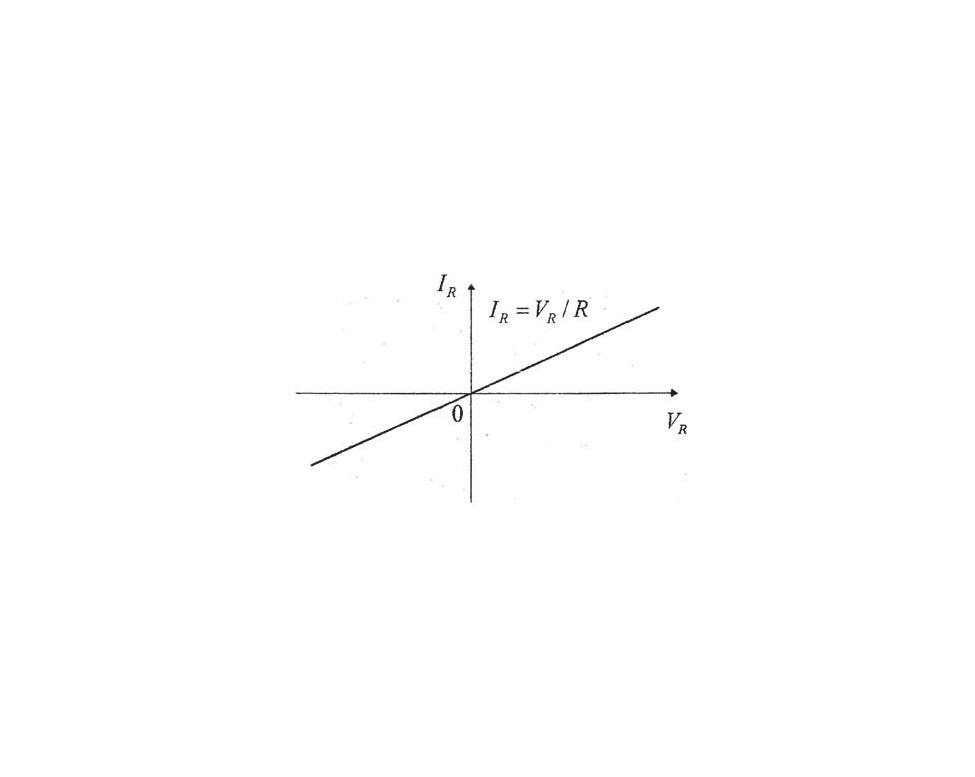
\includegraphics[scale=1]{figurac03.pdf}
    \caption{}
    \label{fig:c.3}
\end{figure}

\end{exmp}

\begin{exmp}
Para el caso de un diodo supuesto ideal, su característica estática será, de acuerdo a su funcionamiento físico, una curva exponencial definida por $I_D=I_S\left(e^{V_D/V_T}-1\right)$. Al medir un diodo real se hallarán desviaciones respecto de la característica idealizada, en las zonas en que no se verifiquen las hipótesis que llevan a la ecuación anterior - figura \ref{fig:c.4} -.

\begin{figure}[!htbp]
    \centering
    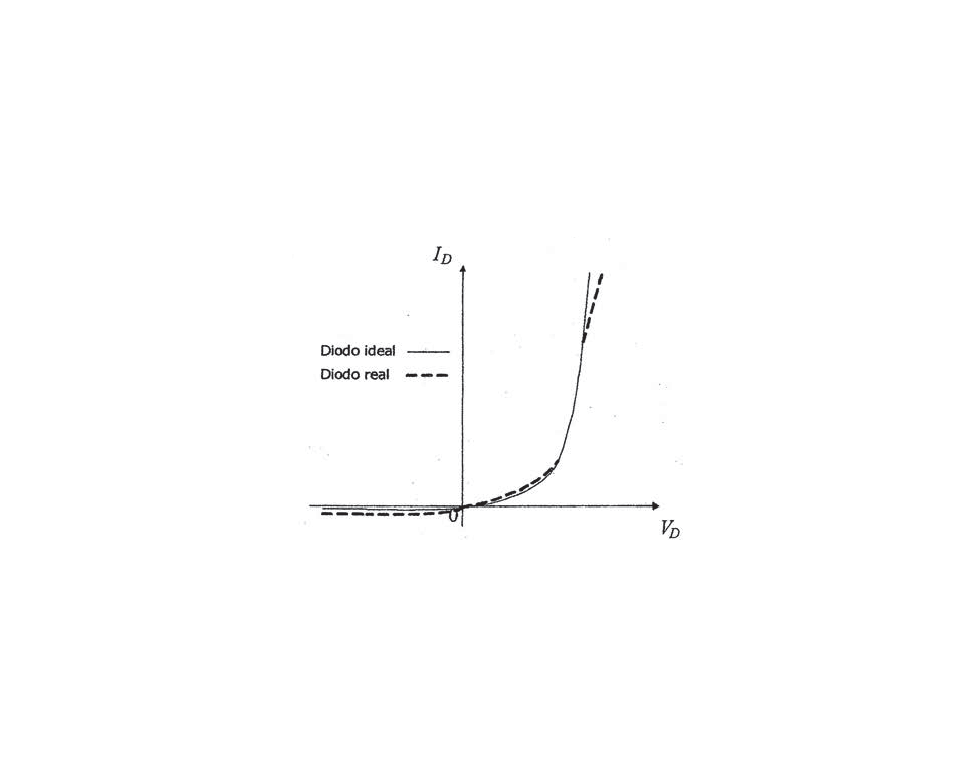
\includegraphics[scale=1]{figurac04.pdf}
    \caption{}
    \label{fig:c.4}
\end{figure}

Tal como se aclaró previamente, debe notarse que por tratarse de una característica estática las capacitancias parásitas u otros efectos reactivos del dispositivo no tienen influencia.
\end{exmp}

\section{Circuitos elementales con Diodos}

\subsection{Circuito serie diodo-resistencia. Análisis estático}

Consideramos un circuito con un diodo polarizado en directa en serie con una resistencia, alimentado por una fuente de tensión continua - figura \ref{fig:c.5} -.

\begin{figure}[!htbp]
\centering
\begin{minipage}{.5\textwidth}
  \centering
  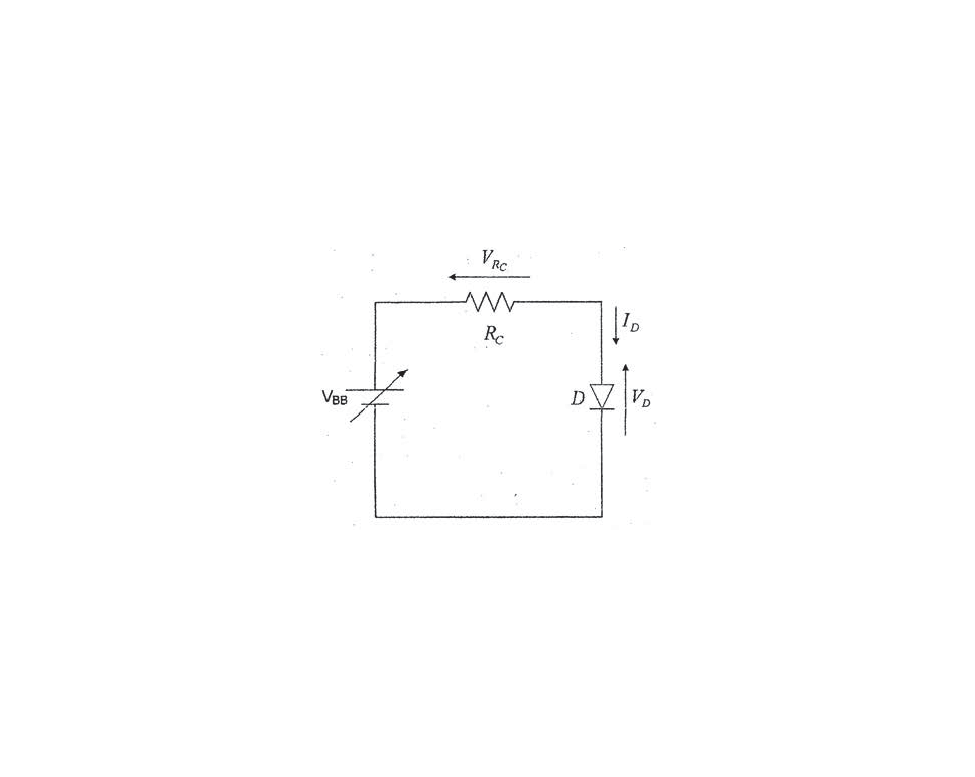
\includegraphics[scale=1]{figurac05.pdf}
  \captionof{figure}{}
  \label{fig:c.5}
\end{minipage}%
\begin{minipage}{.5\textwidth}
  \centering
  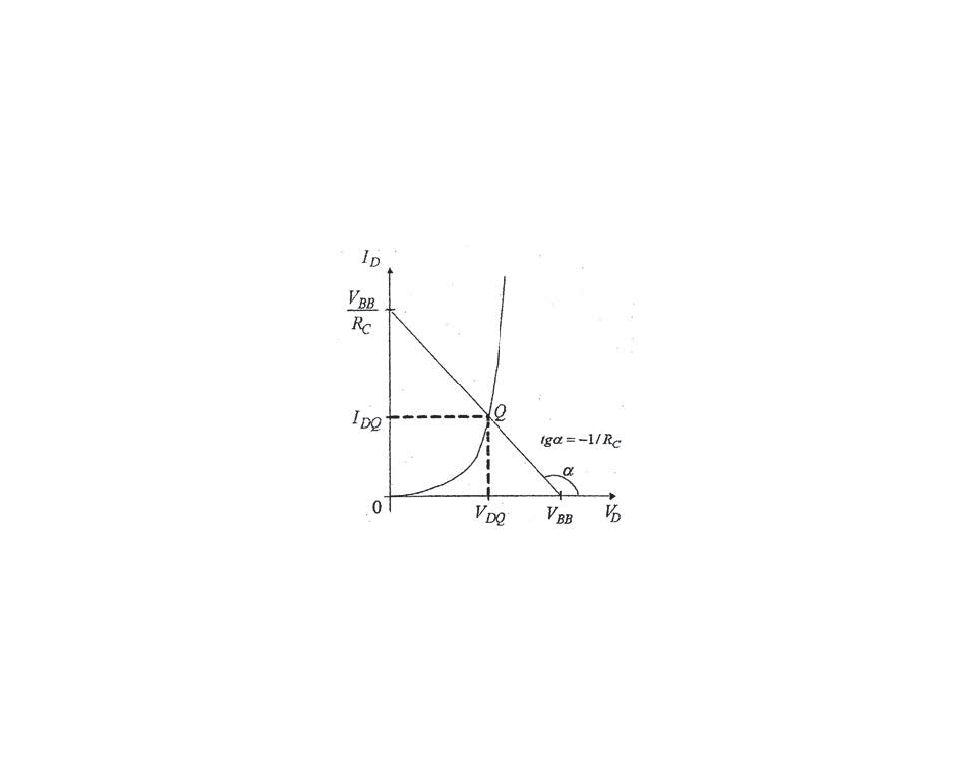
\includegraphics[scale=1]{figurac06.pdf}
  \captionof{figure}{}
  \label{fig:c.6}
\end{minipage}
\end{figure}

Por el circuito circulará una corriente $I_D$, siendo $V_D$ y $V_{RC}$ las diferencia de potencial entre bornes del diodo y de la resistencia, respectivamente. Deberá cumplirse: $V_{BB}=V_{RC}+V_D=I_DR_C+V_D$.

Luego:
\[I_D=(V_{BB}-V_D)/R_C\]

La expresión anterior llevada al plano ($I_D$, $V_D$) constituye la \textbf{recta de carga estática} para el diodo, y que representa el conjunto de pares de valores ($I_D$, $V_D$)  que satisfacen las condiciones de funcionamiento impuestas por los elementos del circuito externos al dispositivo.

De la definición surge que la recta de carga estática no depende del dispositivo - en este caso el diodo- sino de los elementos del circuito externos a él.

La intersección de la recta de carga estática con la característica estática del dispositivo determina el punto de trabajo Q de coordenadas  ($I_{DQ}$, $V_{DQ}$) - figura \ref{fig:c.6} -. 


\subsection{Simplificaciones usuales para el análisis de circuitos con diodos}

\subsubsection{Aproximación de orden cero para la característica estática del diodo}
La ecuación del diodo ideal $I_D=I_S\left(e^{V_D/V_T}-1\right)$ presenta en la zona de polarización directa una pendiente muy pronunciada, y se puede simplificar a $I_D=I_S\e^{V_D/V_T}$ para $V_D>4V_T \simeq 100mV$ (a $25^\circ C$). De modo que para hallar el punto de reposo ($I_{DQ}$, $V_{DQ}$) de un circuito como el de la figura \ref{fig:c.5}, la característica estática del diodo puede ser aproximada por una semirecta horizontal coincidente con el eje de abscisas ($I_D=0$) hasta un valor de tensión $V_K$ conocido como ``tensión de codo'' seguida por otra; ésta vertical, pasando por $V_K$ - figura \ref{fig:c.7}-.

El valor de la tensión de codo se encuentra cerca de los $0.7V$ para diodos de silicio; $0.2V$ para los diodos de germanio y metal-semiconductor (dido Schottky), y entre $1.2V$ y $1.7V$ para los diodos LED.
\begin{figure}[!htbp]
    \centering
    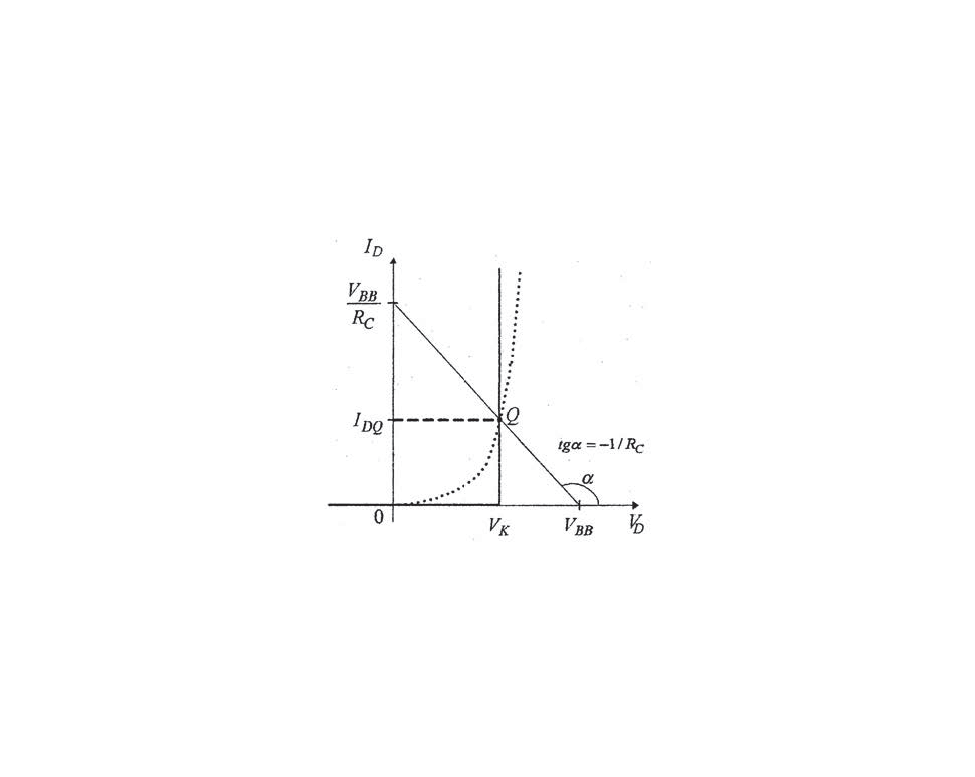
\includegraphics[scale=1]{figurac07.pdf}
    \caption{}
    \label{fig:c.7}
\end{figure}


Este tipo de modelización del diodo es aplicable también en circuitos en lo que el diodo permanece en polarización directa o inversa durante ciertos intervalos de tiempo definidos, ante la aplicación de señales variables de gran amplitud; tales como los recortadores. Se entiende que la denominación de polarización directa o inversa se refiere a cuando está bien definida, es decir suficientemente alejados del origen (por ejemplo, en el caso de diodos de silicio, para valores superiores a $0.5V$ en una u otra polaridad).






\chapter{Trazado de curvas mediante PSpice}
\chapter{Formas de onda en el circuito de salifa de un amplificador básico en emisor común para distintas amplitudes de $v_{be}$ y distintos puntos de reposo}
\chapter{Introducción al funcionamiento de los osciladores}

\end{appendices}

\end{document}
